%%%%%%%%%%%%%%%%%%%%%%%%%%%%%%%%%%%%%%%%%
% Beamer Presentation
% LaTeX Template
% Version 1.0 (10/11/12)
%
% This template has been downloaded from:
% http://www.LaTeXTemplates.com
%
% License:
% CC BY-NC-SA 3.0 (http://creativecommons.org/licenses/by-nc-sa/3.0/)
%
%%%%%%%%%%%%%%%%%%%%%%%%%%%%%%%%%%%%%%%%%

%----------------------------------------------------------------------------------------
%	PACKAGES AND THEMES
%----------------------------------------------------------------------------------------

\documentclass{beamer}

\mode<presentation> {

% The Beamer class comes with a number of default slide themes
% which change the colors and layouts of slides. Below this is a list
% of all the themes, uncomment each in turn to see what they look like.

%\usetheme{default}
%\usetheme{AnnArbor}
%\usetheme{Antibes}
%\usetheme{Bergen}
%\usetheme{Berkeley}
%\usetheme{Berlin}
%\usetheme{Boadilla}
%\usetheme{CambridgeUS}
%\usetheme{Copenhagen}
%\usetheme{Darmstadt}
%\usetheme{Dresden}
%\usetheme{Frankfurt}
%\usetheme{Goettingen}
%\usetheme{Hannover}
%\usetheme{Ilmenau}
%\usetheme{JuanLesPins}
%\usetheme{Luebeck}
\usetheme{Madrid}
%\usetheme{Malmoe}
%\usetheme{Marburg}
%\usetheme{Montpellier}
%\usetheme{PaloAlto}
%\usetheme{Pittsburgh}
%\usetheme{Rochester}
%\usetheme{Singapore}
%\usetheme{Szeged}
%\usetheme{Warsaw}

% As well as themes, the Beamer class has a number of color themes
% for any slide theme. Uncomment each of these in turn to see how it
% changes the colors of your current slide theme.

%\usecolortheme{albatross}
%\usecolortheme{beaver}
%\usecolortheme{beetle}
%\usecolortheme{crane}
%\usecolortheme{dolphin}
%\usecolortheme{dove}
%\usecolortheme{fly}
%\usecolortheme{lily}
%\usecolortheme{orchid}
%\usecolortheme{rose}
%\usecolortheme{seagull}
%\usecolortheme{seahorse}
%\usecolortheme{whale}
%\usecolortheme{wolverine}

%\setbeamertemplate{footline} % To remove the footer line in all slides uncomment this line
%\setbeamertemplate{footline}[page number] % To replace the footer line in all slides with a simple slide count uncomment this line

%\setbeamertemplate{navigation symbols}{} % To remove the navigation symbols from the bottom of all slides uncomment this line
}
\AtBeginSection[]
{
  \begin{frame}<beamer>
    \frametitle{Overview of section \thesection}
    \tableofcontents[currentsection]
  \end{frame}
}
\usepackage{array}
\usepackage{multirow}
\usepackage{graphicx} % Allows including images
\usepackage{booktabs} % Allows the use of \toprule, \midrule and \bottomrule in tables
\newtheorem{thm}{Theorem}
\newtheorem{lem}[thm]{Lemma}
%----------------------------------------------------------------------------------------
%	TITLE PAGE
%----------------------------------------------------------------------------------------

\title[Thesis Defense]{Cellular System Performance Analysis Under Correlated Shadow Fading} % The short title appears at the bottom of every slide, the full title is only on the title page

\author{Tingting Lu} % Your name
\institute[NYU] % Your institution as it will appear on the bottom of every slide, may be shorthand to save space
{
New York University \\ % Your institution for the title page
Tandon School of Engineering\\
\medskip
\textit{tl984@nyu.edu} % Your email address
}
\date{April 17th, 2017} % Date, can be changed to a custom date

\begin{document}
\setbeamertemplate{caption}{\raggedright\insertcaption\par}
\begin{frame}
\titlepage % Print the title page as the first slide
\end{frame}

\begin{frame}
\frametitle{Overview} % Table of contents slide, comment this block out to remove it
\tableofcontents % Throughout your presentation, if you choose to use \section{} and \subsection{} commands, these will automatically be printed on this slide as an overview of your presentation
\end{frame}

%----------------------------------------------------------------------------------------
%	PRESENTATION SLIDES
%----------------------------------------------------------------------------------------

%------------------------------------------------
\section{Motivation} % Sections can be created in order to organize your presentation into discrete blocks, all sections and subsections are automatically printed in the table of contents as an overview of the talk
%------------------------------------------------

\subsection{Why Correlated Shadow Fading} % A subsection can be created just before a set of slides with a common theme to further break down your presentation into chunks
\begin{frame}
\frametitle{Introduction of Fading}
In general, fading can be divided into two categories: large-scale fading and small-scale fading
\begin{itemize}
\item Large-scale fading: shadow fading caused by obstacles (trees, buildings, etc.) in the propagation path.
\item Small-scale fading: caused by multipath propagation.
\end{itemize}
Next Generation Cellular Networks:
\begin{itemize}
\item Millimeter wave (mmWave) frequency spectrum, between 30 and 300 GHz, will most likely be used to address the bandwidth needs.
\item The small wavelengths of mmWave will result in high path loss and sensitivity to obstructions which cause large-scale shadow fading.
\item Shadow fading can lead to significant received power loss over a wide area.
\end{itemize}
%\begin{figure}
%\includegraphics[width=8cm]{fading.png}
%\end{figure}
\end{frame}

\begin{frame}
\frametitle{Correlated Shadow Fading}
\begin{block}{}
In general, shadow fading is approximated by an independent log-normal distribution with a standard deviation derived from empirical measurements.
\end{block}
\begin{block}{}
This model fails to capture the spatial correlations in shadow fading.
\end{block}
\begin{columns}[c]
\column{.3\textwidth}
A mobile user moving behind a row of tall buildings.
\column{.7\textwidth}
\begin{figure}
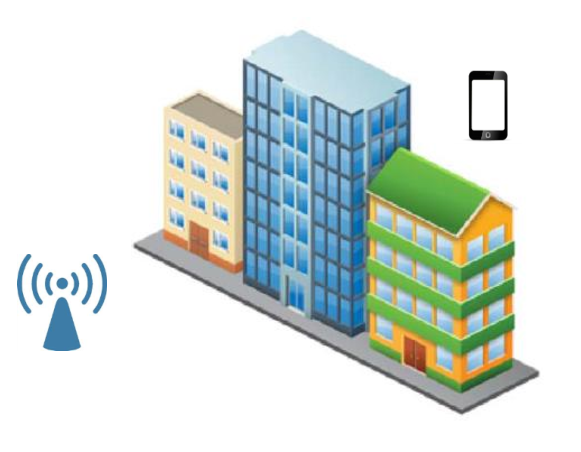
\includegraphics[width=5cm]{building.eps}
\end{figure}
\end{columns}
\end{frame}
%
%
%\subsection{Shadow Fading Correlation Models}
\begin{frame}
\frametitle{Shadow Fading Correlation Models}
Specific Correlation Models:
\begin{itemize}
\item Constant Model
\item Absolute Distance-Only Models: Exponential Model
\item Angle-Only Models
\item Separable Models: Angle-Distance Ratio and Angle-Absolute Distance
\end{itemize}
Autocorrelation and Cross-Correlation:
\begin{figure}
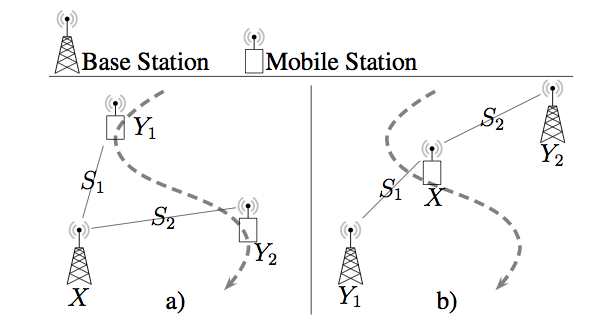
\includegraphics[width=8cm]{AutoandCross.png}
\end{figure}
\end{frame}
%

\section{Cooperative Communication for a Single-Cell Model}
\subsection{Angular and Distance Correlation Model}
\begin{frame}
\frametitle{Angular and Distance Correlation Model}
We consider a correlation model involves both angular and distance as follows:
\begin{equation}
\theta = |\angle\vec{r_{i}}-\angle\vec{r_{j}}|\in [0^{\circ},180^{\circ}],
\end{equation}
\begin{equation}
R=|10\log_{10}r_{i}/r_{j}|=\frac{10}{\ln 10}|\ln r_{i}-\ln r_{j}|,
\end{equation}
\begin{equation}
h(\vec{r_{i}},\vec{r_{j}})=max\{1-\theta/\theta_{0},0\}\cdot max\{1-R/R_{0},0\}.
\end{equation}
\begin{figure}
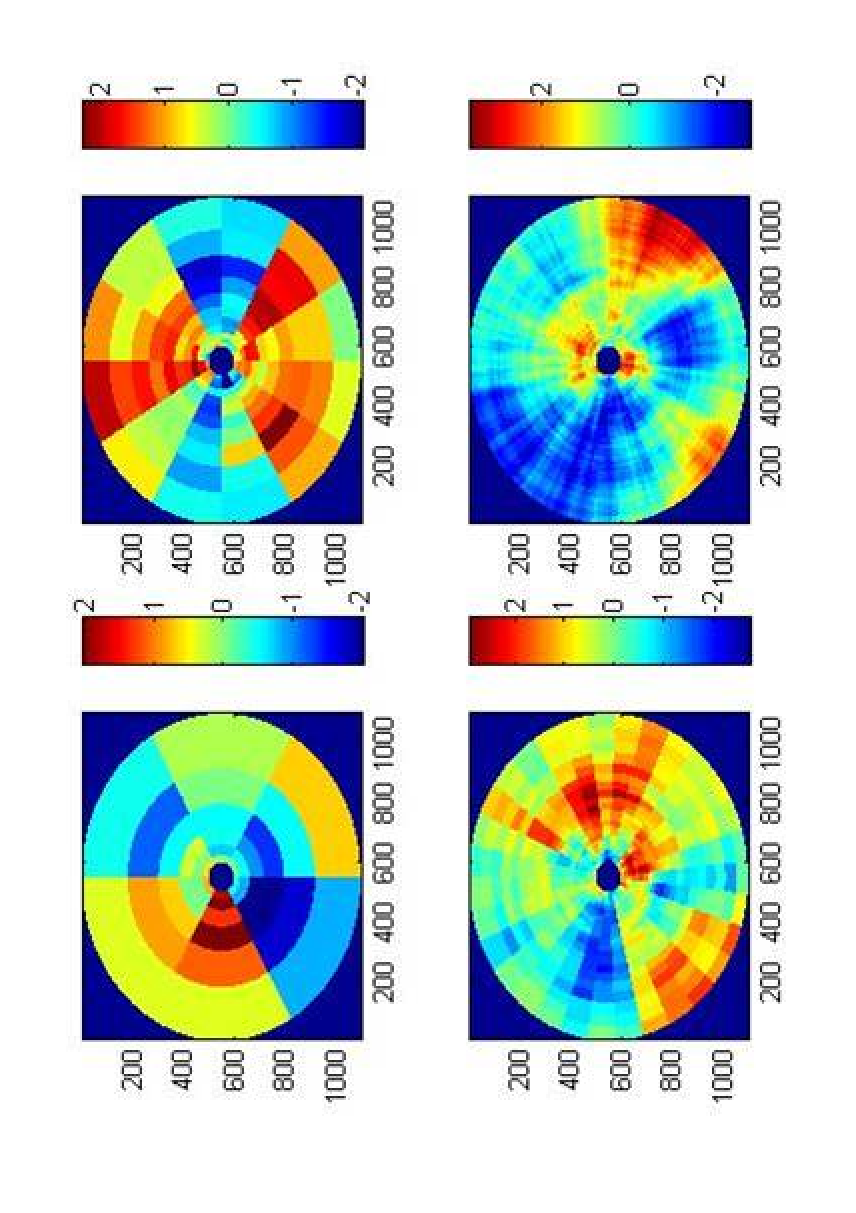
\includegraphics[width=3cm, angle=270]{shadowingfield_V3.eps}
\caption{Correlated Shadowing Fields for Increasing Resolutions}
\end{figure}
\end{frame}
%\subsection{Correlated Outage Fields}
\begin{frame}
\frametitle{Correlated Outage Fields}
\begin{figure}
\centering
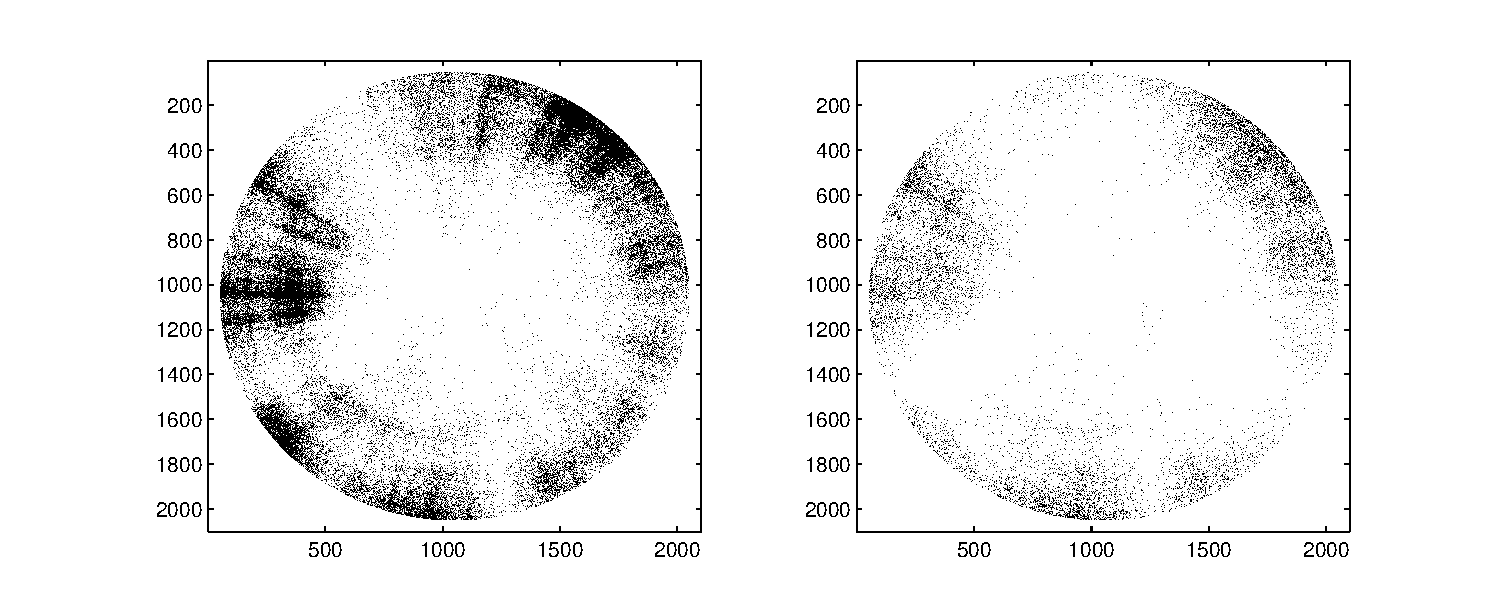
\includegraphics[width=8cm]{outagefield.eps}
\caption{Correlated Outage Fields (Dark areas are outage areas while white areas are non-outage areas)}
\label{outagefie}
\end{figure}
\end{frame}
%
\subsection{How Cooperative Communication Mitigate Shadow Fading}
\begin{frame}
\frametitle{System Model}
A single cell cellular deployment.
\begin{figure}
\centering
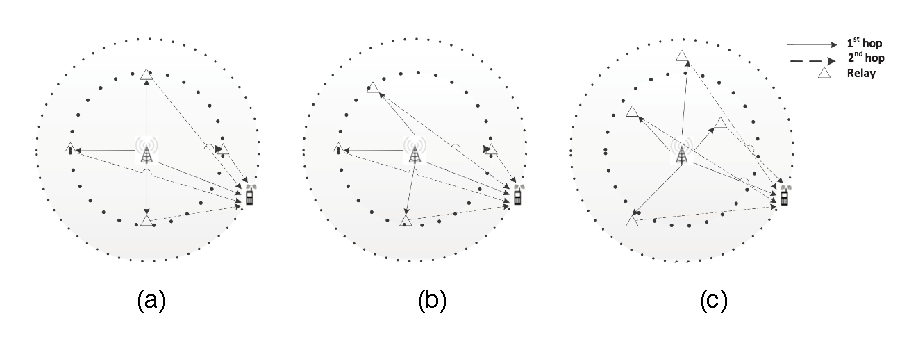
\includegraphics[width=9cm]{abc.eps}
\caption{System Model and Three Different Relay Placements}
\label{threemodels}
\end{figure}
\begin{itemize}
\item Relays are placed uniformly on a circle near the cell edge.
\item Relays are randomly spaced on a circle near the cell edge.
\item Relays are placed randomly in the cell.
\end{itemize}
\end{frame}
%
\begin{frame}
\frametitle{Cooperative Communication Scheme}
\begin{itemize}
\item First Hop: BS broadcasts signals to both relays and MS. If MS receives and decodes the signals transmitted by BS successfully, there is no need for relays to repeat the transmission. If not, relays which successfully decode the signals will participate in the second hop retransmission. Relays which cannot decode the received signal successfully, will not participate in the second hop.
\item Second Hop: Among all relays which participate in the second hop, the one that has the best channel gain between the relay and MS will be chosen (this can be done by centralized control or using information from pilot signals). This relay will encode the signals again and send the coded bits to the MS.
\end{itemize}
\end{frame}
%
%\begin{frame}
%\frametitle{Outage Probability Analysis}
%In the first hop, relays that can successfully decode the signals transmitted from BS is a subset $\mathcal{R}_{n}$ of $N$ relays defined by:
%\begin{equation}
%\mathcal{R}_{n}\triangleq \{ i: \log_{2}(1+\text{SNR}_{S-i})\ge R\},
%\end{equation}
%where $\text{SNR}_{S-i}$ is the received signal-to-noise ratio from BS to relay $i$ and $n\in\{0,1,\cdots,2^{N}\}$.\\
%In the second hop, the selected best relay $j$ is the relay in $\mathcal{R}_{n}$ that has the maximum SNR among all relays in $\mathcal{R}_{n}$, i.e., $j=\arg\max_{i\in \mathcal{R}_{n}}\{\text{SNR}_{i-D}\}$ where $\text{SNR}_{i-D}$ denotes the SNR from the $i$th relay to the destination MS. The BS to MS SNR is denoted by $\text{SNR}_{S-D}$. 
%\end{frame}
%
%\begin{frame}
%\frametitle{Outage Probability Analysis Cont'd}
%\begin{itemize}
%\item The probability that an MS cannot receive signals directly from the BS successfully:
%\begin{equation}
%P_{out_{0}} = P[\text{SNR}_{S-D}<\gamma],
%\end{equation}
%\item The outage event happens in the first hop if no relay can receive the signal from the BS successfully, which means $\mathcal{R}_{0}=\phi$.
%\begin{equation}
%P_{out_{1}} = \max_{i = 1,\cdots,N} P[\text{SNR}_{S-i}<\gamma].
%\end{equation}
%\item If the outage does not happen in the first hop, then the outage event may happen in the second hop with probability:
%\begin{equation}
%P_{out_{2}} = \sum_{n=1,\cdots,2^{N}}P[\text{SNR}_{j-D}<\gamma|\mathcal{R}_{n}]P[\mathcal{R}_{n}],
%\end{equation}
%where $j$ is the index of the relay which has the best channel gain between it and the MS.
%\end{itemize}
%\end{frame}

\begin{frame}
\frametitle{Outage Probability of the System}
 The outage probability of the system:
\begin{equation}
P_{out_{S}} = P_{out_{0}}*(P_{out_{1}}+(1-P_{out_{1}})*P_{out_{2}}).
\end{equation}
\end{frame}
%%
%\begin{frame}
%\frametitle{How to Calculate the Outage Probability}
%The probability density function (pdf) of shadow fading $S$ given $L$ correlated fading branches is
%\begin{equation}
%\begin{split}
%f_{\mathbf{S}}(\mathbf{s}) = &\frac{\lambda^{L}}{\sqrt{2\pi}|\mathbf{K}_{L\times L}|^{1/2}\prod_{i=1}^{L}s_{i}}\\
%&\cdot\exp(-\frac{1}{2}(10\log_{10}\mathbf{s}-\mathbf{\mu})^{T}\mathbf{K}_{L\times L}^{-1}(10\log_{10}\mathbf{s}-\mathbf{\mu})),
%\end{split}
%\end{equation}
%where $\lambda = 10/\ln10$ and $\mathbf{\mu}$ is the average shadow fading which is normally $0$. $\mathbf{K}_{L\times L}$ is the correlation matrix. 
%\end{frame}
%
%\begin{frame}
%\frametitle{How to Calculate the Outage Probability (Cont'd)}
%Given $\mathcal{R}_{0}=\phi$ and let $\gamma_{ai}$ denotes the shadow fading threshold for the $i$th relay in the $a$th hop where $a=0,1,2$, where the $0$th hop is the direct transmission from BS to MS, we then have
%\begin{equation}
%P_{out_{1}} = \underbrace{\int_{-\infty}^{+\infty}\cdots\int_{-\infty}^{+\infty}}_{i =1,\cdots,N}\prod g_{0}(\gamma_{1i})f(\mathbf{s_{1}})d\mathbf{s_{1}}.
%\end{equation}
%For $n=1,\cdots,2^{N}$, the outage probability for the second hop is
%\begin{equation}
%\begin{split}
%P_{out_{2}} = \sum_{n=1,\cdots,2^{N}}\underbrace{\int_{-\infty}^{+\infty}\cdots\int_{-\infty}^{+\infty}}_{i=1,\cdots,N}\prod g_{n}(\gamma_{1i}) f(\mathbf{s_{1}})d\mathbf{s_{1}}\\
%\cdot\underbrace{\int_{-\infty}^{+\infty}\cdots\int_{-\infty}^{+\infty}}_{i\in \mathcal{R}_{n}}\prod g_{n}(\gamma_{2i})f(\mathbf{s_{2}})d\mathbf{s_{2}},
%\end{split}
%\end{equation}
%\end{frame}
%
%\begin{frame}
%\frametitle{How to Calculate the Outage Probability (Cont'd)}
%where $\mathbf{s_{1}}$ is the correlated shadow fading in the first hop, $\mathbf{s_{2}}$ is the correlated shadow fading in the second hop, $u$ is a step function and
%\begin{equation}
%g_{n}(\gamma_{ai}) = \{\begin{array}{cc}
%               u(\gamma_{ai}) & i\in \mathcal{R}_{n} \\
%               1-u(\gamma_{ai}) & i\notin \mathcal{R}_{n}
%             \end{array}.
%\end{equation}
%\begin{figure}
%\centering
%\includegraphics[width=6cm]{theo_vs_simu_V2.eps}
%\caption{Theoretical and Simulated Outage Probability for Mode 1}
%\label{theovssimu}
%\end{figure}
%\end{frame}
%
\begin{frame}
\frametitle{Simulation and Performance Evaluation}
\begin{table}
\centering
\caption{\label{SystemConfig}Simulation Configuration Parameters}

\begin{tabular}{|c|c|}

\hline

\multirow{3}{*}{Okuruma-Hata Model} & BS Height: $100m$\\
& Relay Height: $10m$\\
& MS Height: $1.5m$\\
\hline
%Rayleigh Fading & Coherence Time: $100ms$\\
%\hline
\multirow{4}{*}{Correlated Shadow Fading} & $R_{0}: 6$\\
& $\theta_{0}: \pi /3$\\
& $d_{min}: 50m$\\
\hline
\multirow{2}{*}{Relay Placements} & Three Modes with Density:\\
& 2,4,6,8,10,12\\
\hline
Cell Size & $R: 1000m$\\
\hline
MS Moving Speed & $v: 10m/s$\\
\hline
Radio Frequency & $f: 900MHz$\\
\hline
BS Transmission Power & $P: 26dbm$\\
\hline
SNR Requirement & $8dB$\\
\hline
\end{tabular}

\end{table}
\end{frame}
%
\begin{frame}
\frametitle{Simulation Results and Analysis}
\begin{columns}[c]
\column{.5\textwidth}
\begin{figure}
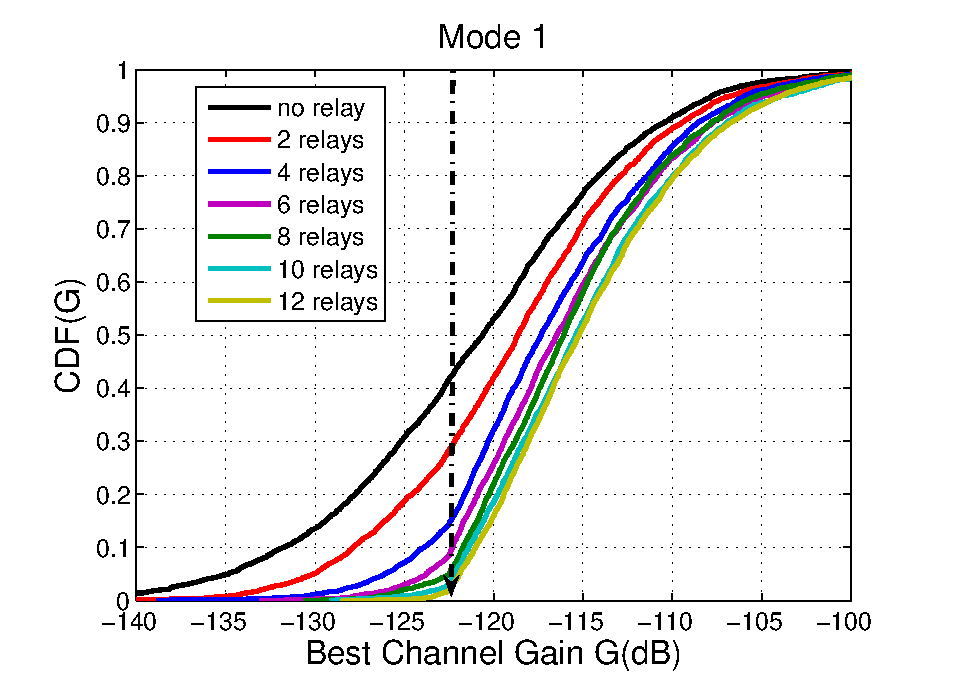
\includegraphics[width=4.5cm]{Mode1_bestchannelgain_V2.eps}
\label{Mode1}
\end{figure}
\begin{figure}
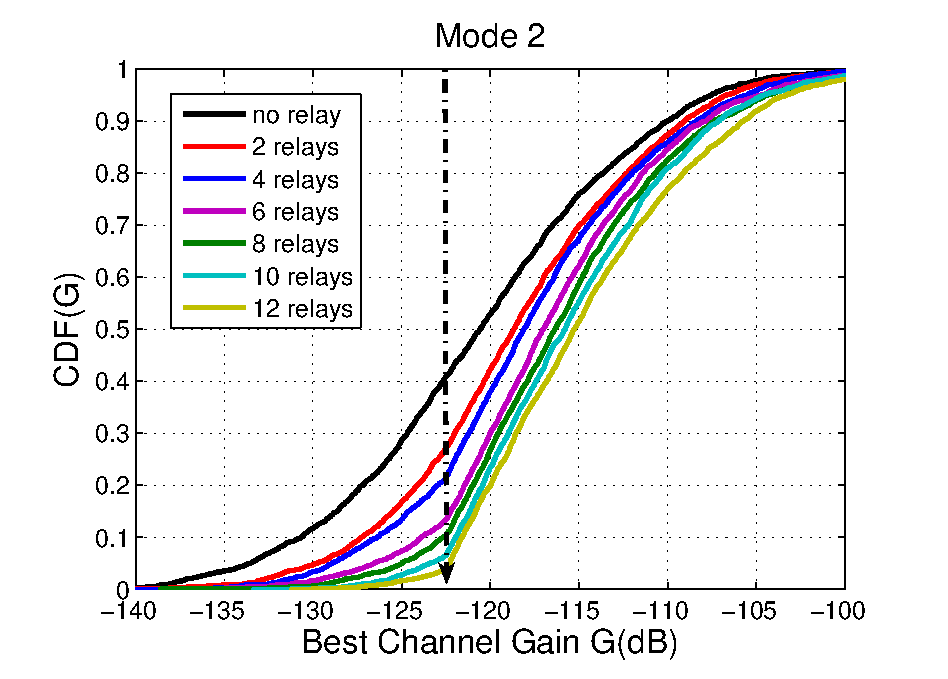
\includegraphics[width=4.5cm]{Mode2_bestchannelgain_V2.eps}
\label{Mode2}
\end{figure}
\column{.5\textwidth}
\begin{figure}
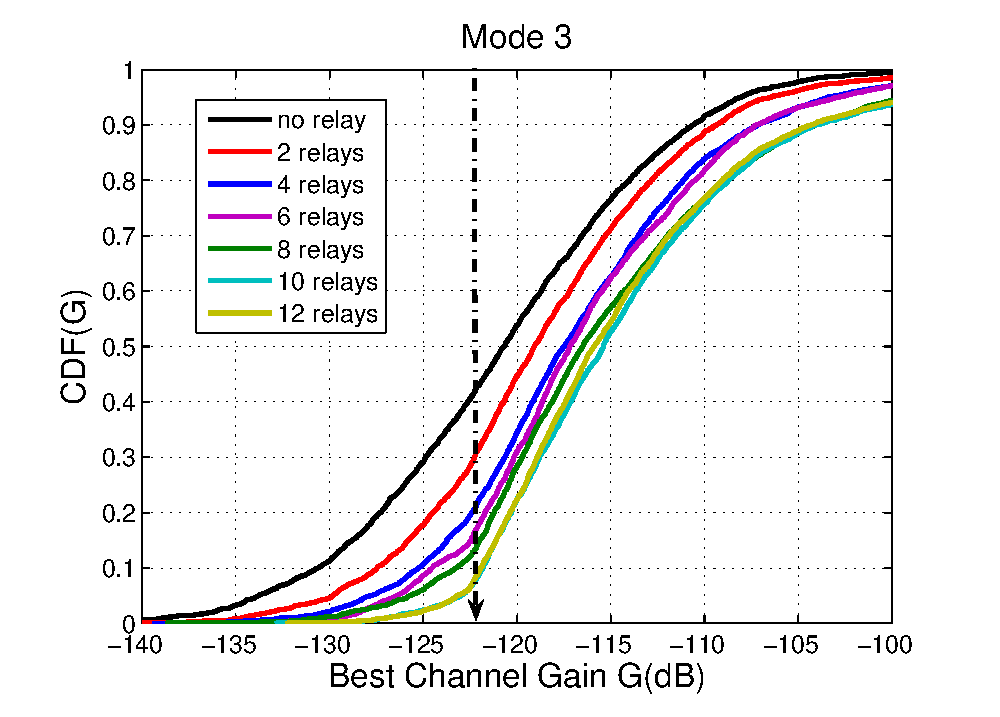
\includegraphics[width=4.5cm]{Mode3_bestchannelgain_V2.eps}
\label{Mode3}
\end{figure}
Best Channel Condition between MS and BS or Relays (corresponding to three different relay deployment modes and several different relay densities. Dashed arrow demonstrates the channel condition that satisfies the SNR requirement.
\end{columns}
\end{frame}

\begin{frame}
\frametitle{Outage Duration}
\begin{columns}[c]
\column{.5\textwidth}
\begin{figure}
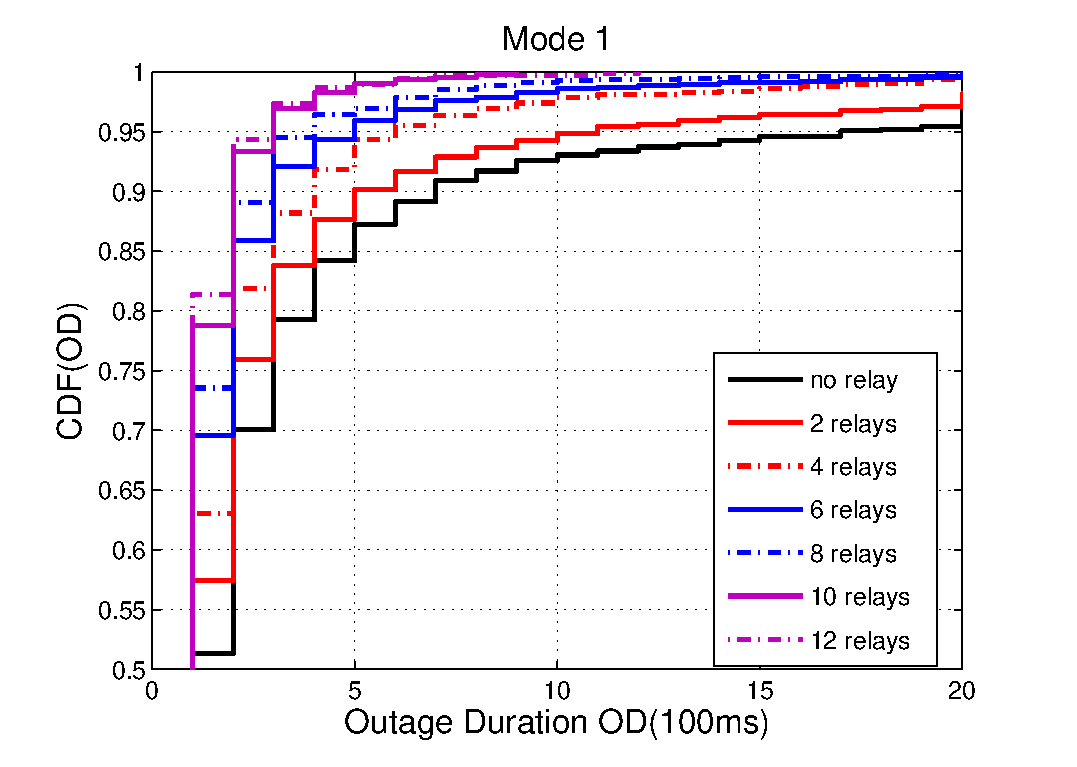
\includegraphics[width=4.5cm]{OutageDuration_Rayleigh_Mode1_V2.eps}
\label{Mode1}
\end{figure}
\begin{figure}
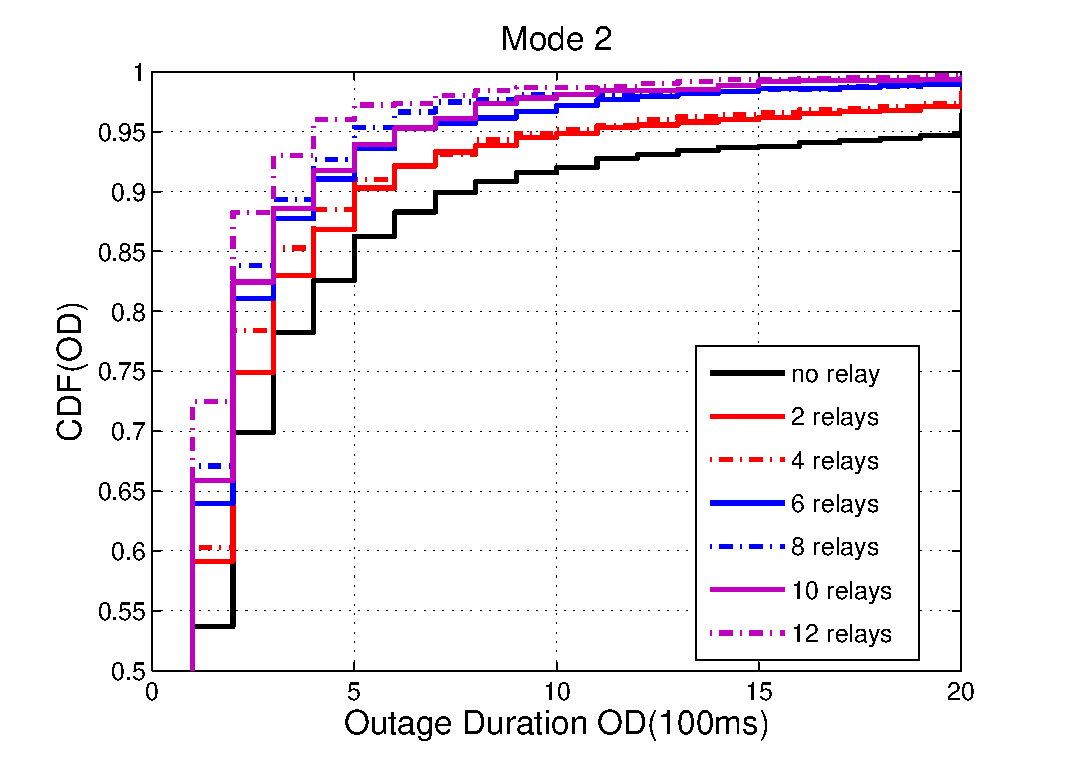
\includegraphics[width=4.5cm]{OutageDuration_Rayleigh_Mode2_V2.eps}
\label{Mode2}
\end{figure}
\column{.5\textwidth}
\begin{figure}
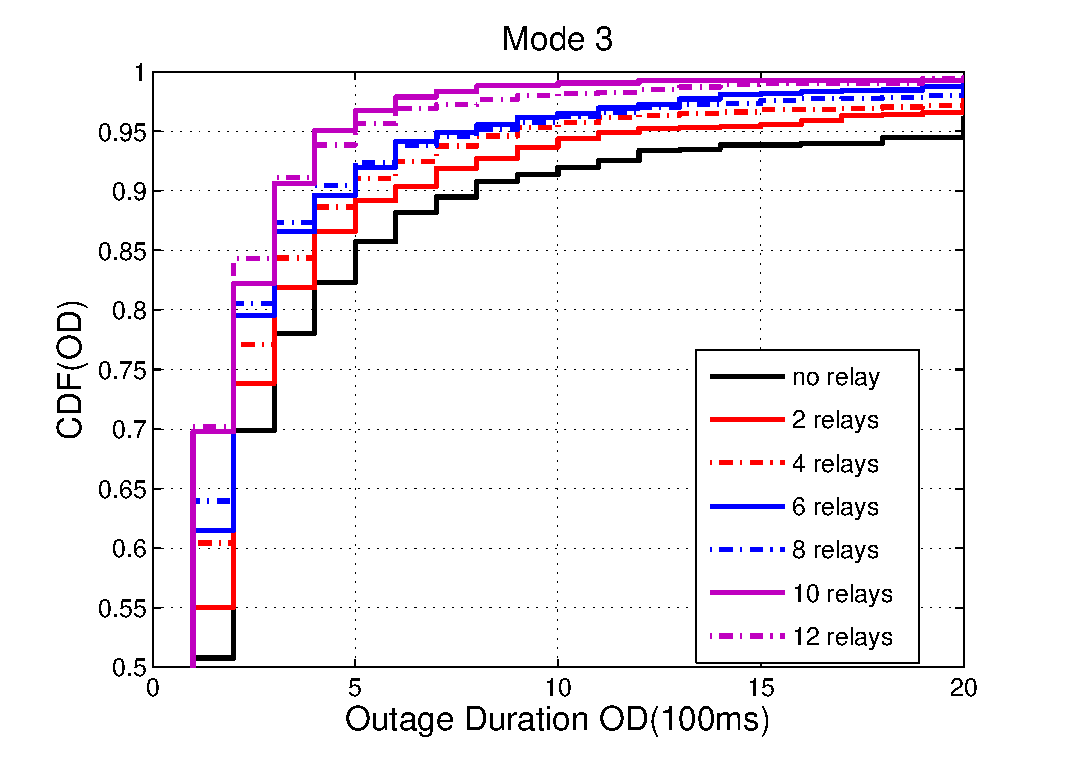
\includegraphics[width=4.5cm]{OutageDuration_Rayleigh_Mode3_V2.eps}
\label{Mode3}
\end{figure}
Cumulative Distribution Function of Outage Duration (with Rayleigh fading)
\end{columns}
\end{frame}

\begin{frame}
\frametitle{Outage Frequency}
\begin{equation}
f_{outage}=\frac{\text{Total Number of Outage Points}}{\text{Total Number of Simulation Points}}.
\end{equation}
\begin{figure}
\centering
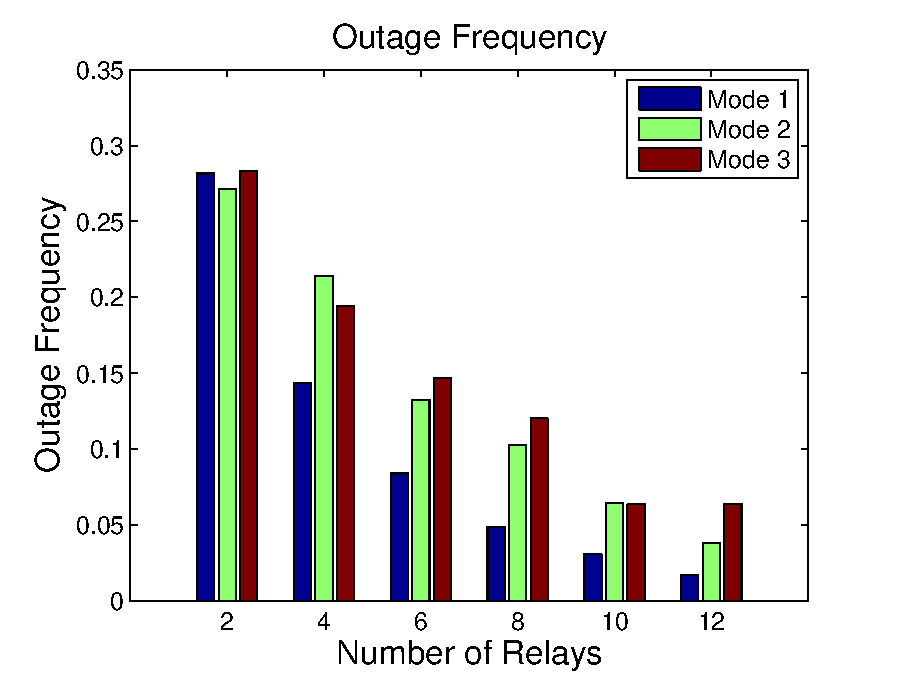
\includegraphics[width=8cm]{outagefrequency_V2.eps}
\label{outagefrequency}
\end{figure}
\end{frame}
%


%\begin{frame}
%\frametitle{Physical Rules}
%\begin{figure}
%\includegraphics[width=6cm]{figure1.png}
%\end{figure}
%\begin{itemize}
%\item $h(\vec{r_{i}},\vec{r_{j}})\approx1$ for $\vec{r_{i}}\approx\vec{r_{j}}$.
%\item $h(\vec{r_{i}},\vec{r_{j}})\ll1$ for $\lVert\vec{r_{i}}-\vec{r_{j}}\rVert\gg0$.
%\item $h$ should be a non increasing function in $\theta$ and $d$.
%\item $h$ should be nonnegative.
%\item $h$ should be small for large $\theta$ and approach zero for $\theta\approx180^{o}$, and $r_{1}$ and $r_{2}$ large.
%\item Continuity: a small change in $\vec{r_{i}}$ should result in small changes in $h(\vec{r_{i}},\vec{r_{j}})$.
%\end{itemize}
%\end{frame}
%
%
\section{Single-Cell System Performance Analysis}

%\subsection{Why Exponential Correlation Model}
\begin{frame}
\frametitle{Exponential Correlation Model}
Exponential correlation model is an analytical model proposed by Gudmundson based on empirical measurements of $900MHz$ frequency.
\begin{equation}
\rho = e^{-\frac{d}{d_{0}}}
\end{equation}
\begin{itemize}
\item Derived from empirical measurements.
\item Does not violated physical rules.
\item Correlation matrix is positive semi-dedifinite.
\item Can be modeled as a first-order autoregressive process spatially.
\item Has low simulation complexity.
\end{itemize}
\begin{block}{Disadvantage}
The correlation is only decided by $d$, $\theta$ is ignored.
\end{block}
\end{frame}
\subsection{First-Order Markov Chain Model}
\begin{frame}
\frametitle{Exponential Correlated Shadowing Field}
\begin{figure}
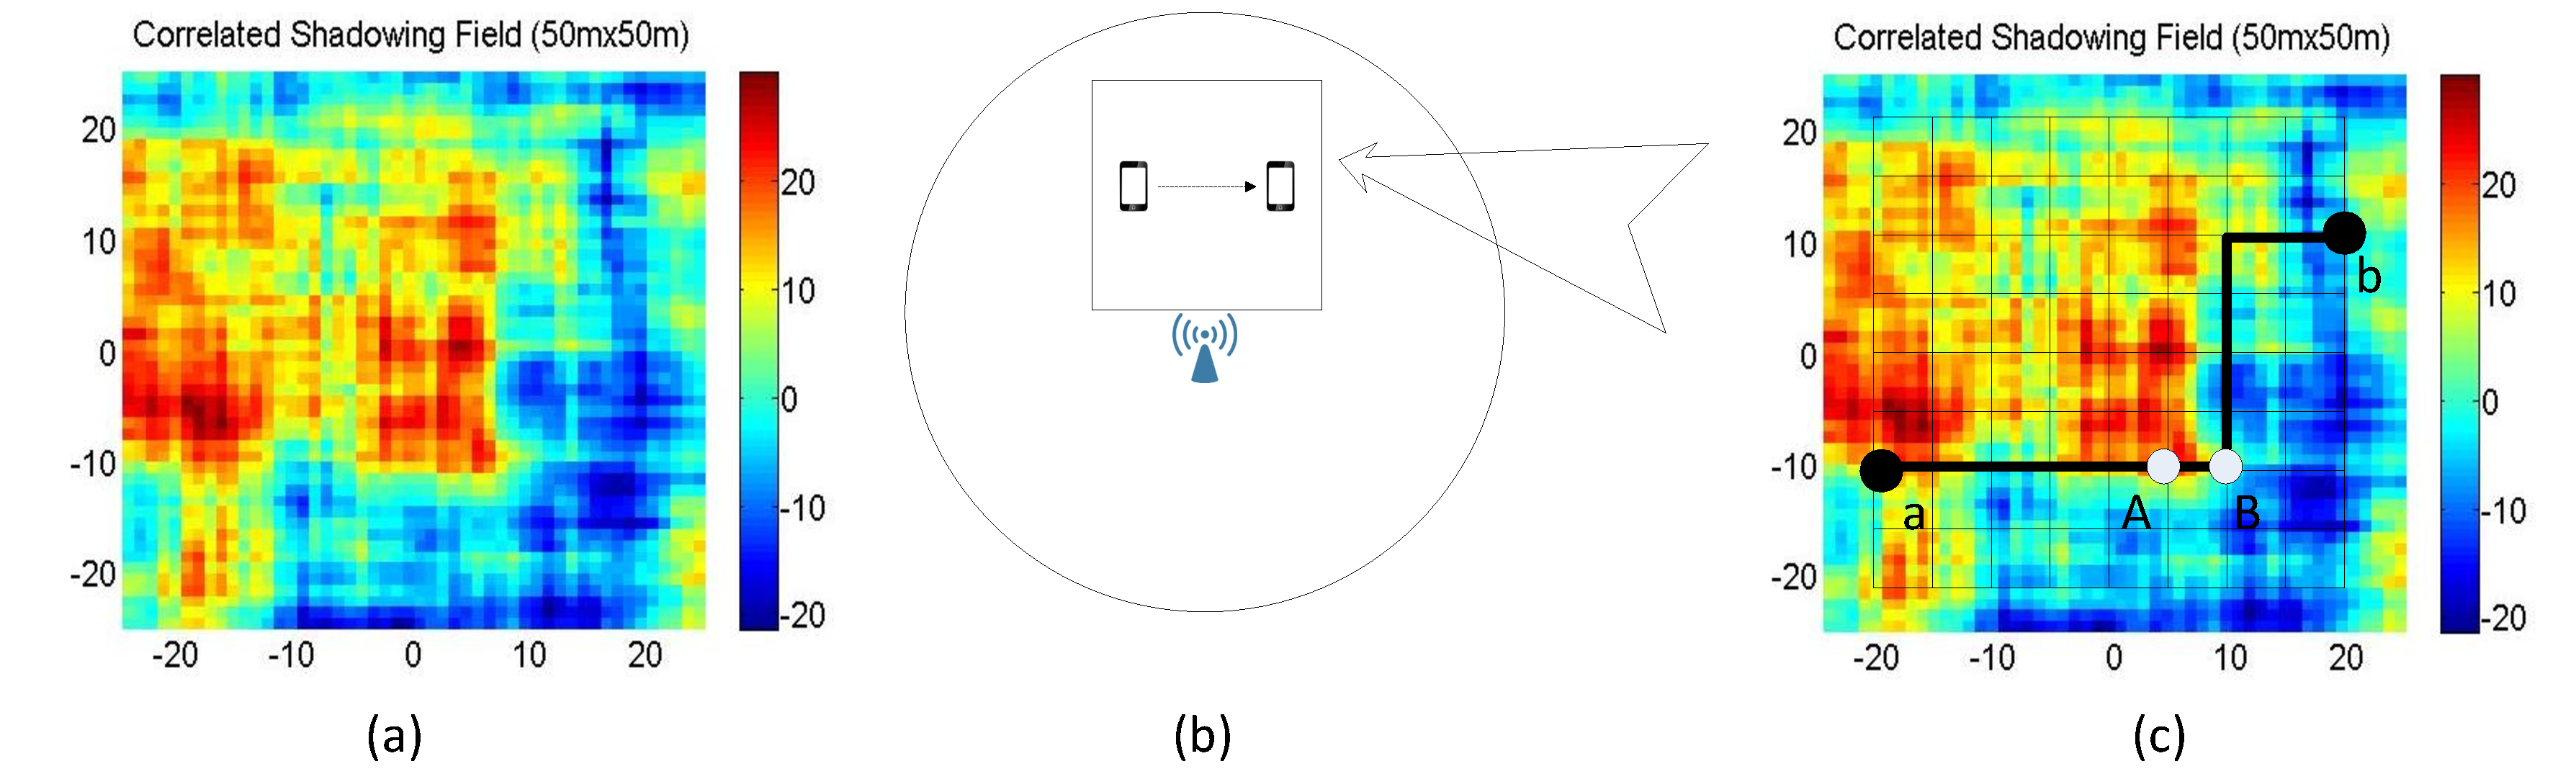
\includegraphics[width=12cm]{finalsystemab_V3.eps}
\caption{(a) A typical exponential correlated shadow fading field in a $50m\times50m$ area. The color bar denotes the value of the shadow fading in dB. (b) A single cell model with a MS moving on a fixed trajectory. The shadow fading field covered the entire trajectory is generated locally. (c) A locally generated correlated shadowing field for a fixed trajectory from point a to point b.}
\end{figure}
\end{frame}
%
\begin{frame}
\frametitle{Exponential Correlation}
$A$ and $B$ are two neighboring points. Assume the shadow fading (in dB) is $N(0,\sigma^{2})$.\\
The spatial correlation between $S_{A}$ and $S_{B}$ is:
\begin{equation}
\rho_{A,B} = \frac{E[S_{A}S_{B}]}{\sigma^{2}}=e^{-\frac{d_{A,B}}{d_{0}}}
\end{equation}
This can be written as:
\begin{equation}
S_{B}=\rho S_{A}+(1-\rho)n_{A}
\end{equation}
where $n_{A}$ denotes the channel noise at $A$.
\end{frame}
%
%\begin{frame}
%\frametitle{First-Order Markov Chain Model}
%\begin{lem}
%Shadow fading factors of any two points that can be connected by a trajectory have jointly gaussian distribution.
%\end{lem}
%\begin{proof}Suppose the two points are $a$ and $b$, we can assume there are $n$ positions on this trajectory $(t_{1},t_{2},\dots,t_{n})$. Then we have the following:
%\begin{equation}
%\begin{split}
%S_{b} &=\rho S_{t_{n}}+(1-\rho)e_{t_{n}}\\
%&=\rho(\rho S_{t_{n-1}}+(1-\rho)e_{t_{n-1}})+(1-\rho)e_{t_{n}}=\ldots\ldots\\
%&=\rho^{n}S_{t_{1}}+\sum_{i=1}^{n}\rho^{n-i}(1-\rho)e_{t_{i}}\\
%&=\rho^{n+1}S_{a}+\rho(1-\rho)e_{a}+\sum_{i=1}^{n}\rho^{n-i}(1-\rho)e_{t_{i}}
%\end{split}
%\end{equation}
%\end{proof}
%\end{frame}
%
%\begin{frame}
%\frametitle{Proof Cont'd}
%\begin{proof}
%Let $X=\alpha S_{a}+\beta S_{b}$, the following can be derived:
%\begin{equation}
%X=\alpha S_{a}+\beta(\rho^{n+1}S_{a}+\rho(1-\rho)e_{a}+\sum_{i=1}^{n}\rho^{n-i}(1-\rho)e_{t_{i}})
%\end{equation}
%Since $S_{a}$, $e_{t_{i}}$ and $e_{a}$ are all independent and Gaussian random variables, we conclude that $X$ is also Gaussian, which implies that $S_{a}$ and $S_{b}$ are jointly Gaussian.
%\end{proof}
%\end{frame}

\begin{frame}
\frametitle{Construct Markov Chain Model}
\begin{lem}
Shadow fading factors of any two points that can be connected by a trajectory have jointly gaussian distribution.
\end{lem}
\begin{itemize}
\item Divide the entire shadow fading range $[-\infty,+\infty]$ into finite number of intervals $\{[-\infty,S_{0}],[S_{0},S_{1}],\dots,[S_{N},+\infty]\}$. Each interval represents a state of the Markov chain model.
\item Derive the state transition matrix of the Markov chain model from the probability distribution of the correlated shadow fading.
\item Derive the steady-state probability from the state transition matrix of the Markov chain model.
\end{itemize}
\end{frame}
%
\begin{frame}
\frametitle{State Transition Matrix}
Assume there are $N$ states of the Markov chain model $ST_{1}, ST_{2},\cdots, ST_{N}$ where $ST_{i}$ corresponds to interval $(S_{i-1}, S_{i}]$. Then we have the state transition probability as follows:
\begin{equation}
\label{statetransition}
\begin{split}
P_{i,j} &= P(S_{A}\in ST_{j}|S_{B}\in ST_{i})\\
&=\frac{P(S_{A}\in ST_{j}, S_{B}\in ST_{i})}{P(S_{B}\in ST_{i})}\\
&=\frac{\int_{S_{i-1}}^{S_{i}}(\int_{S_{j-1}}^{S_{j}}f_{(S_{A}|S_{B}=s_{B}}(s_{A})ds_{A})f(s_{B})ds_{B}}{\int_{S_{i-1}}^{S_{i}}f(s_{B})ds_{B}}
\end{split}
\end{equation}
\end{frame}
%
\subsection{Analysis of Outage Behavior}
%\begin{frame}
%\frametitle{Outage Behavior}
%The received signal on a link $(S\to D)$ between source and destination is given by:
% \begin{equation}
%y_{D} = G_{SD}x_{S}+n_{D}.
%\end{equation}
%End-to-end received signal-to-noise ratio (SNR) is:
%\begin{equation}
%\text{SNR} \triangleq P*G_{SD}^{2}/N_{0}
%\end{equation}
%Outage happens when $G_{SD}^2 < \beta$, where $\beta = \frac{(2^{R}-1)*N_{0}}{P}$ and $R$ is the required data rate. 
%\end{frame}
%
\begin{frame}
\frametitle{Outage Behavior}
Considering two consecutive points $A$ and $B$, we have $G_{A}=PL_{A}(d_{A})+S_{A}$ and $G_{B}=PL_{B}(d_{B})+S_{B}$. The probability of $A$ and $B$ are both in outage area can be written as:
\begin{equation}
\begin{split}
&P(G_{A}<\gamma, G_{B}<\gamma) \\
&= P(S_{A}<\gamma-PL_{A}(d_{A}), S_{B}<\gamma-PL_{B}(d_{B}))
\end{split}
\end{equation}
If $S_{A}<\gamma-PL_{A}(d_{A}) \in ST_{i}$ and $S_{B}<\gamma-PL_{B}(d_{B}) \in ST_{j}$, we can infer that, to avoid outage, the lower bound of shadow fading factor $S_{A}$ is in state $ST_{i}$ and for $S_{B}$ is in state $ST_{j}$. State $ST_{i}$ and $ST_{j}$ are called lower bound state. 
\end{frame}
%
\begin{frame}
\frametitle{Outage Behavior Cont'd}
\begin{equation}
P(G_{A}<\gamma, G_{B}<\gamma)=\sum_{m=0}^{i}\sum_{n=0}^{j} P(ST_{m})\bullet P(ST_{m},ST_{n})
\end{equation}
\begin{equation}
\begin{split}
&P(G_{1}<\gamma,\dots,G_{L}<\gamma)=\\
&\sum_{m_{1}=0}^{M_{1}}\dots\sum_{m_{L}=0}^{M_{L}} P(ST_{m_{1}})\bullet P(ST_{m_{1}},ST_{m_{2}})\\
&\bullet\dots\bullet P(ST_{m_{L-1}},ST_{m_{L}})
\end{split}
\end{equation}
where $m_{i}$, $i\in\{1,\dots,L\}$ are corresponding lower bound state of each position on the moving trajectory.
\end{frame}
%
%\begin{frame}
%\frametitle{Outage Behavior}
%\begin{table}
%\centering
%\caption{\label{SystemConfig}Simulation Configuration Parameters}
%
%\begin{tabular}{|c|c|}
%
%\hline
%
%\multirow{2}{*}{Okuruma-Hata Model} & BS Height: $100m$\\
%& MS Height: $1m$\\
%\hline
%Rayleigh Fading & Coherence Time: $100ms$\\
%\hline
%\multirow{5}{*}{Correlated Shadow Fading}
%& De-Correlation Distance $d_{0}$: $20m$\\
%& Standard Deviation $\sigma_{0}$: $8dB$\\
%\hline
%\multirow{3}{*}{Markov Chain Model} & Number of States:\\
%& 50, 26, 18, 14, 10, 8\\
%& ($3*\sigma_{0}/n*2+2$, $n=1,2,3,4,6,8$)\\
%\hline
%\multirow{2}{*}{MS Trajectory} & Length: $21m$\\
%& Unit Distance $\delta d$: $1m$\\
%\hline
%Shadowing Field & $50\times50m^{2}$\\
%\hline
%Radio Frequency & $f: 1024MHz$\\
%\hline
%BS Transmission Power & $P: 30dbm$\\
%\hline
%SNR Requirement & $10dB$\\
%\hline
%\end{tabular}
%\end{table}
%\end{frame}
%
\begin{frame}
\begin{figure}
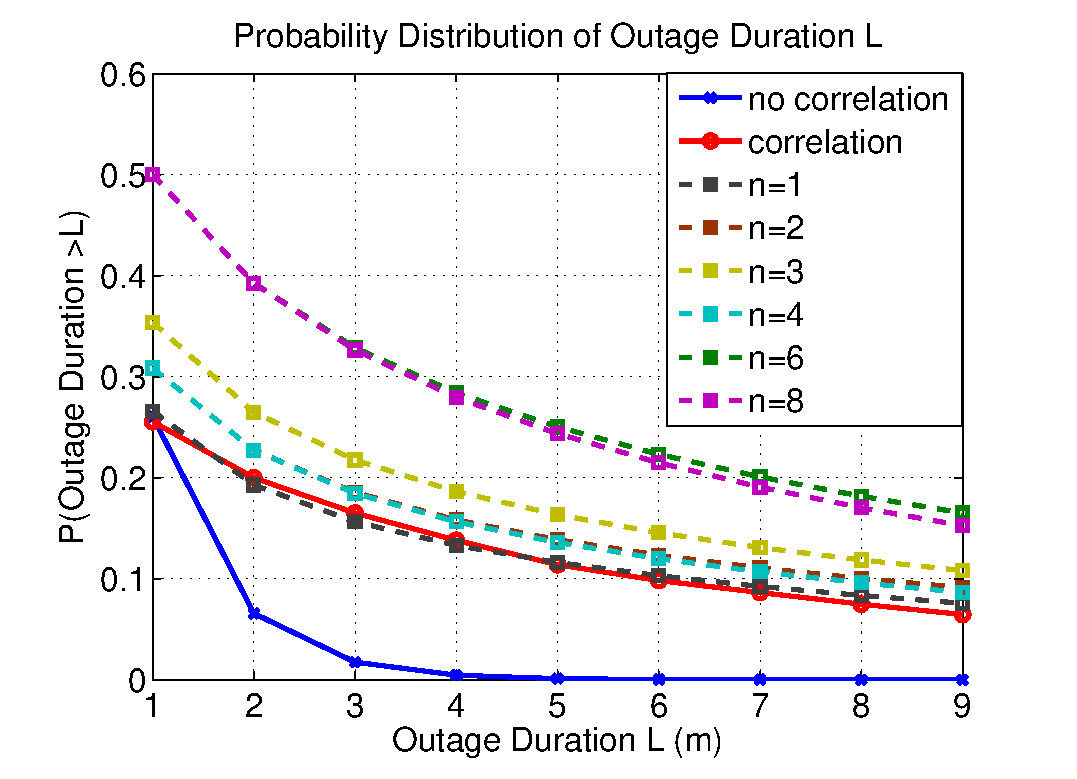
\includegraphics[width=12cm]{result_Plot.eps}
\caption{Probabilities of outage duration greater than $L$.}
\end{figure}
\end{frame}
%
\section{Multi-Cell System Performance Analysis}
\subsection{Grid Model vs. Random Model}
\begin{frame}
\frametitle{Multi-Cell System Model}
\begin{itemize}
 \item Grid Model: $\lambda$ BSs are placed on a regular grid deterministically.
 \item Random Model: $\lambda$ BSs are placed randomly in a fixed area.
\end{itemize}
 \begin{figure}
 \centering
 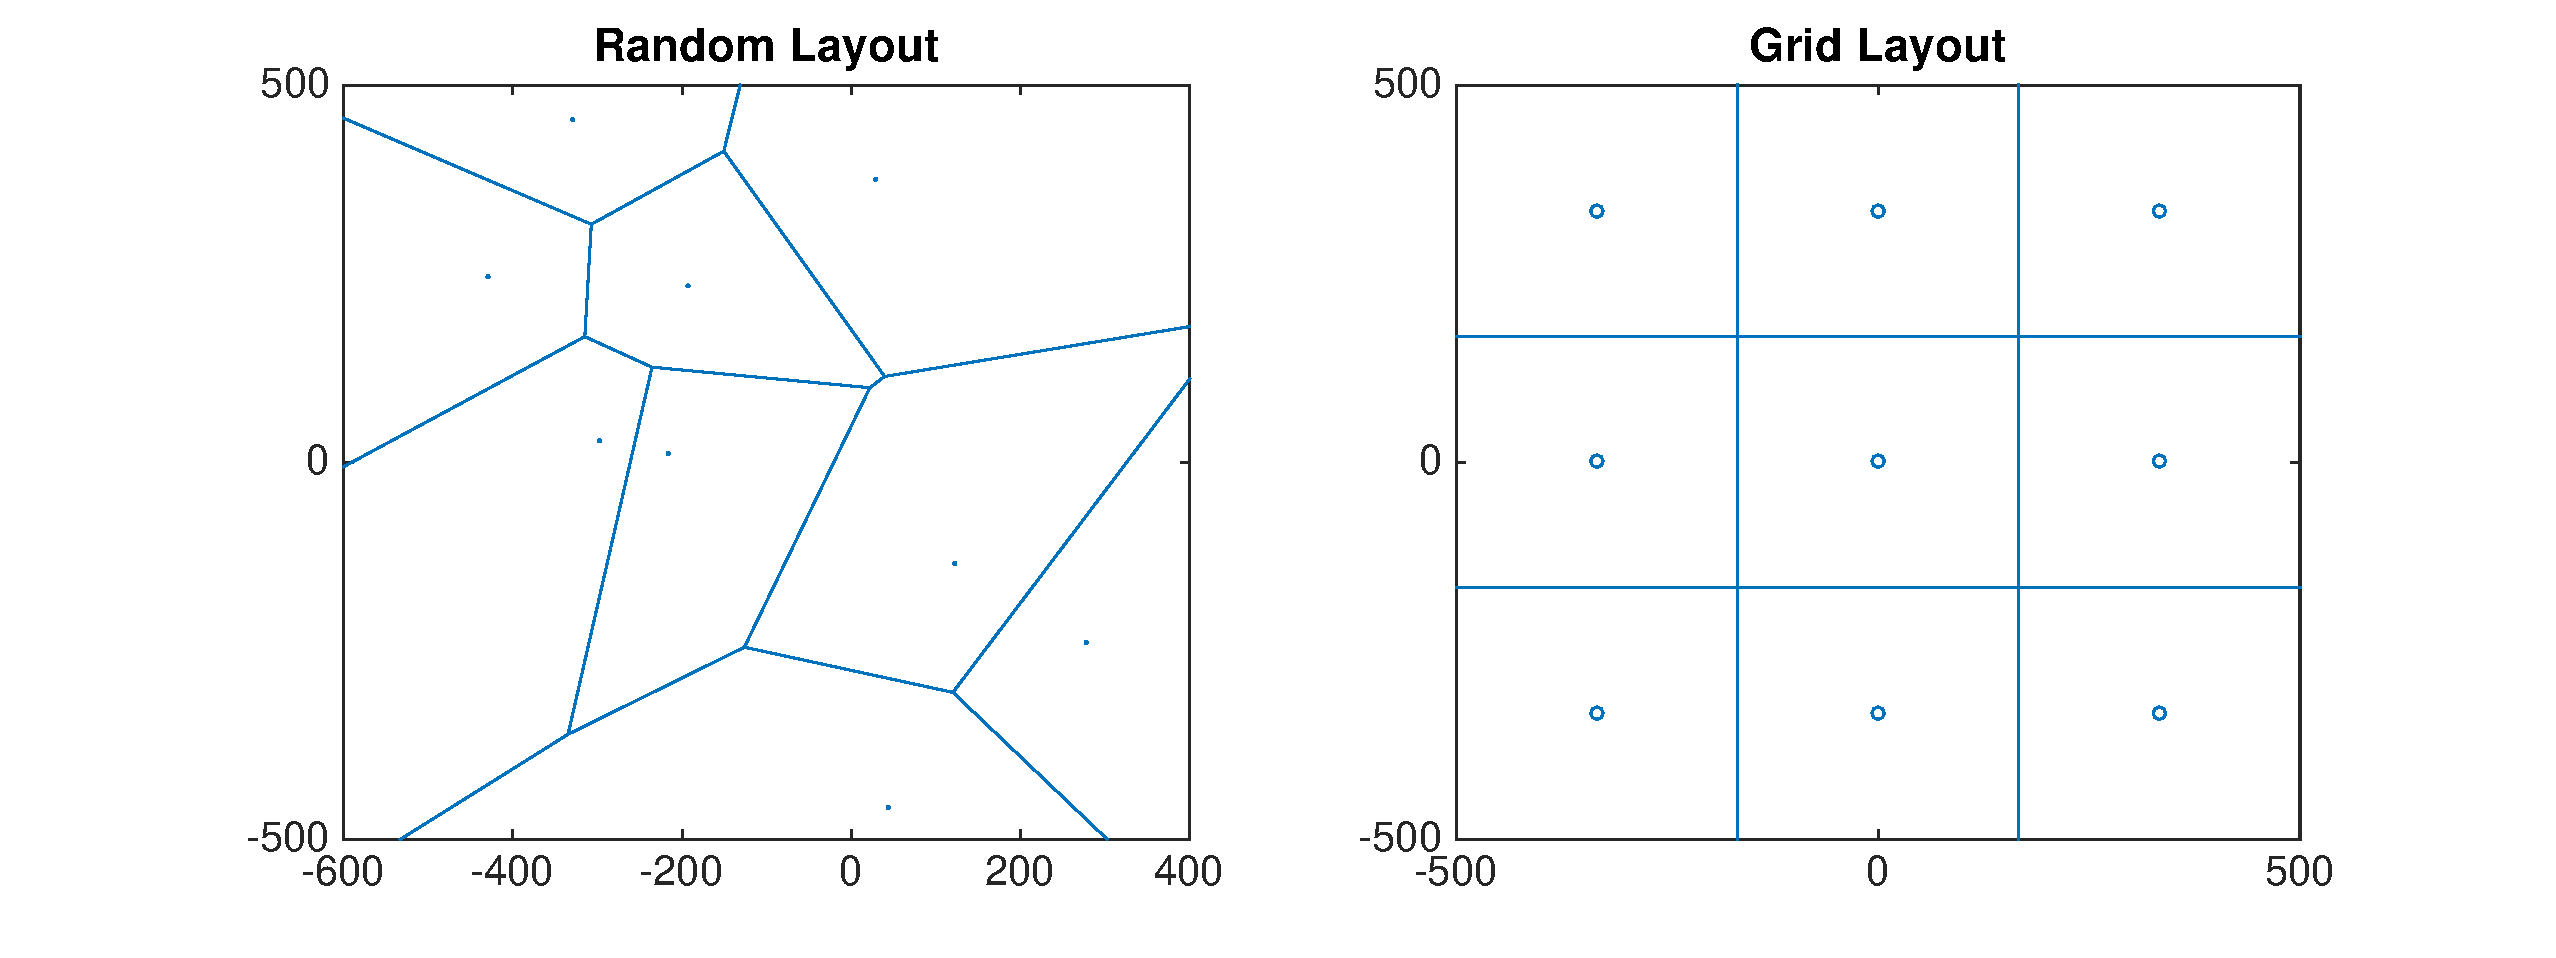
\includegraphics[width=10cm]{systemLayout.eps}
 \caption{Random model and Grid model with $\lambda = 9$.}
 \end{figure}
\end{frame}
\begin{frame}
\frametitle{Grid Model vs. Random Model}
\begin{columns}[c]
\column{.5\textwidth}
 \begin{figure}
 \centering
 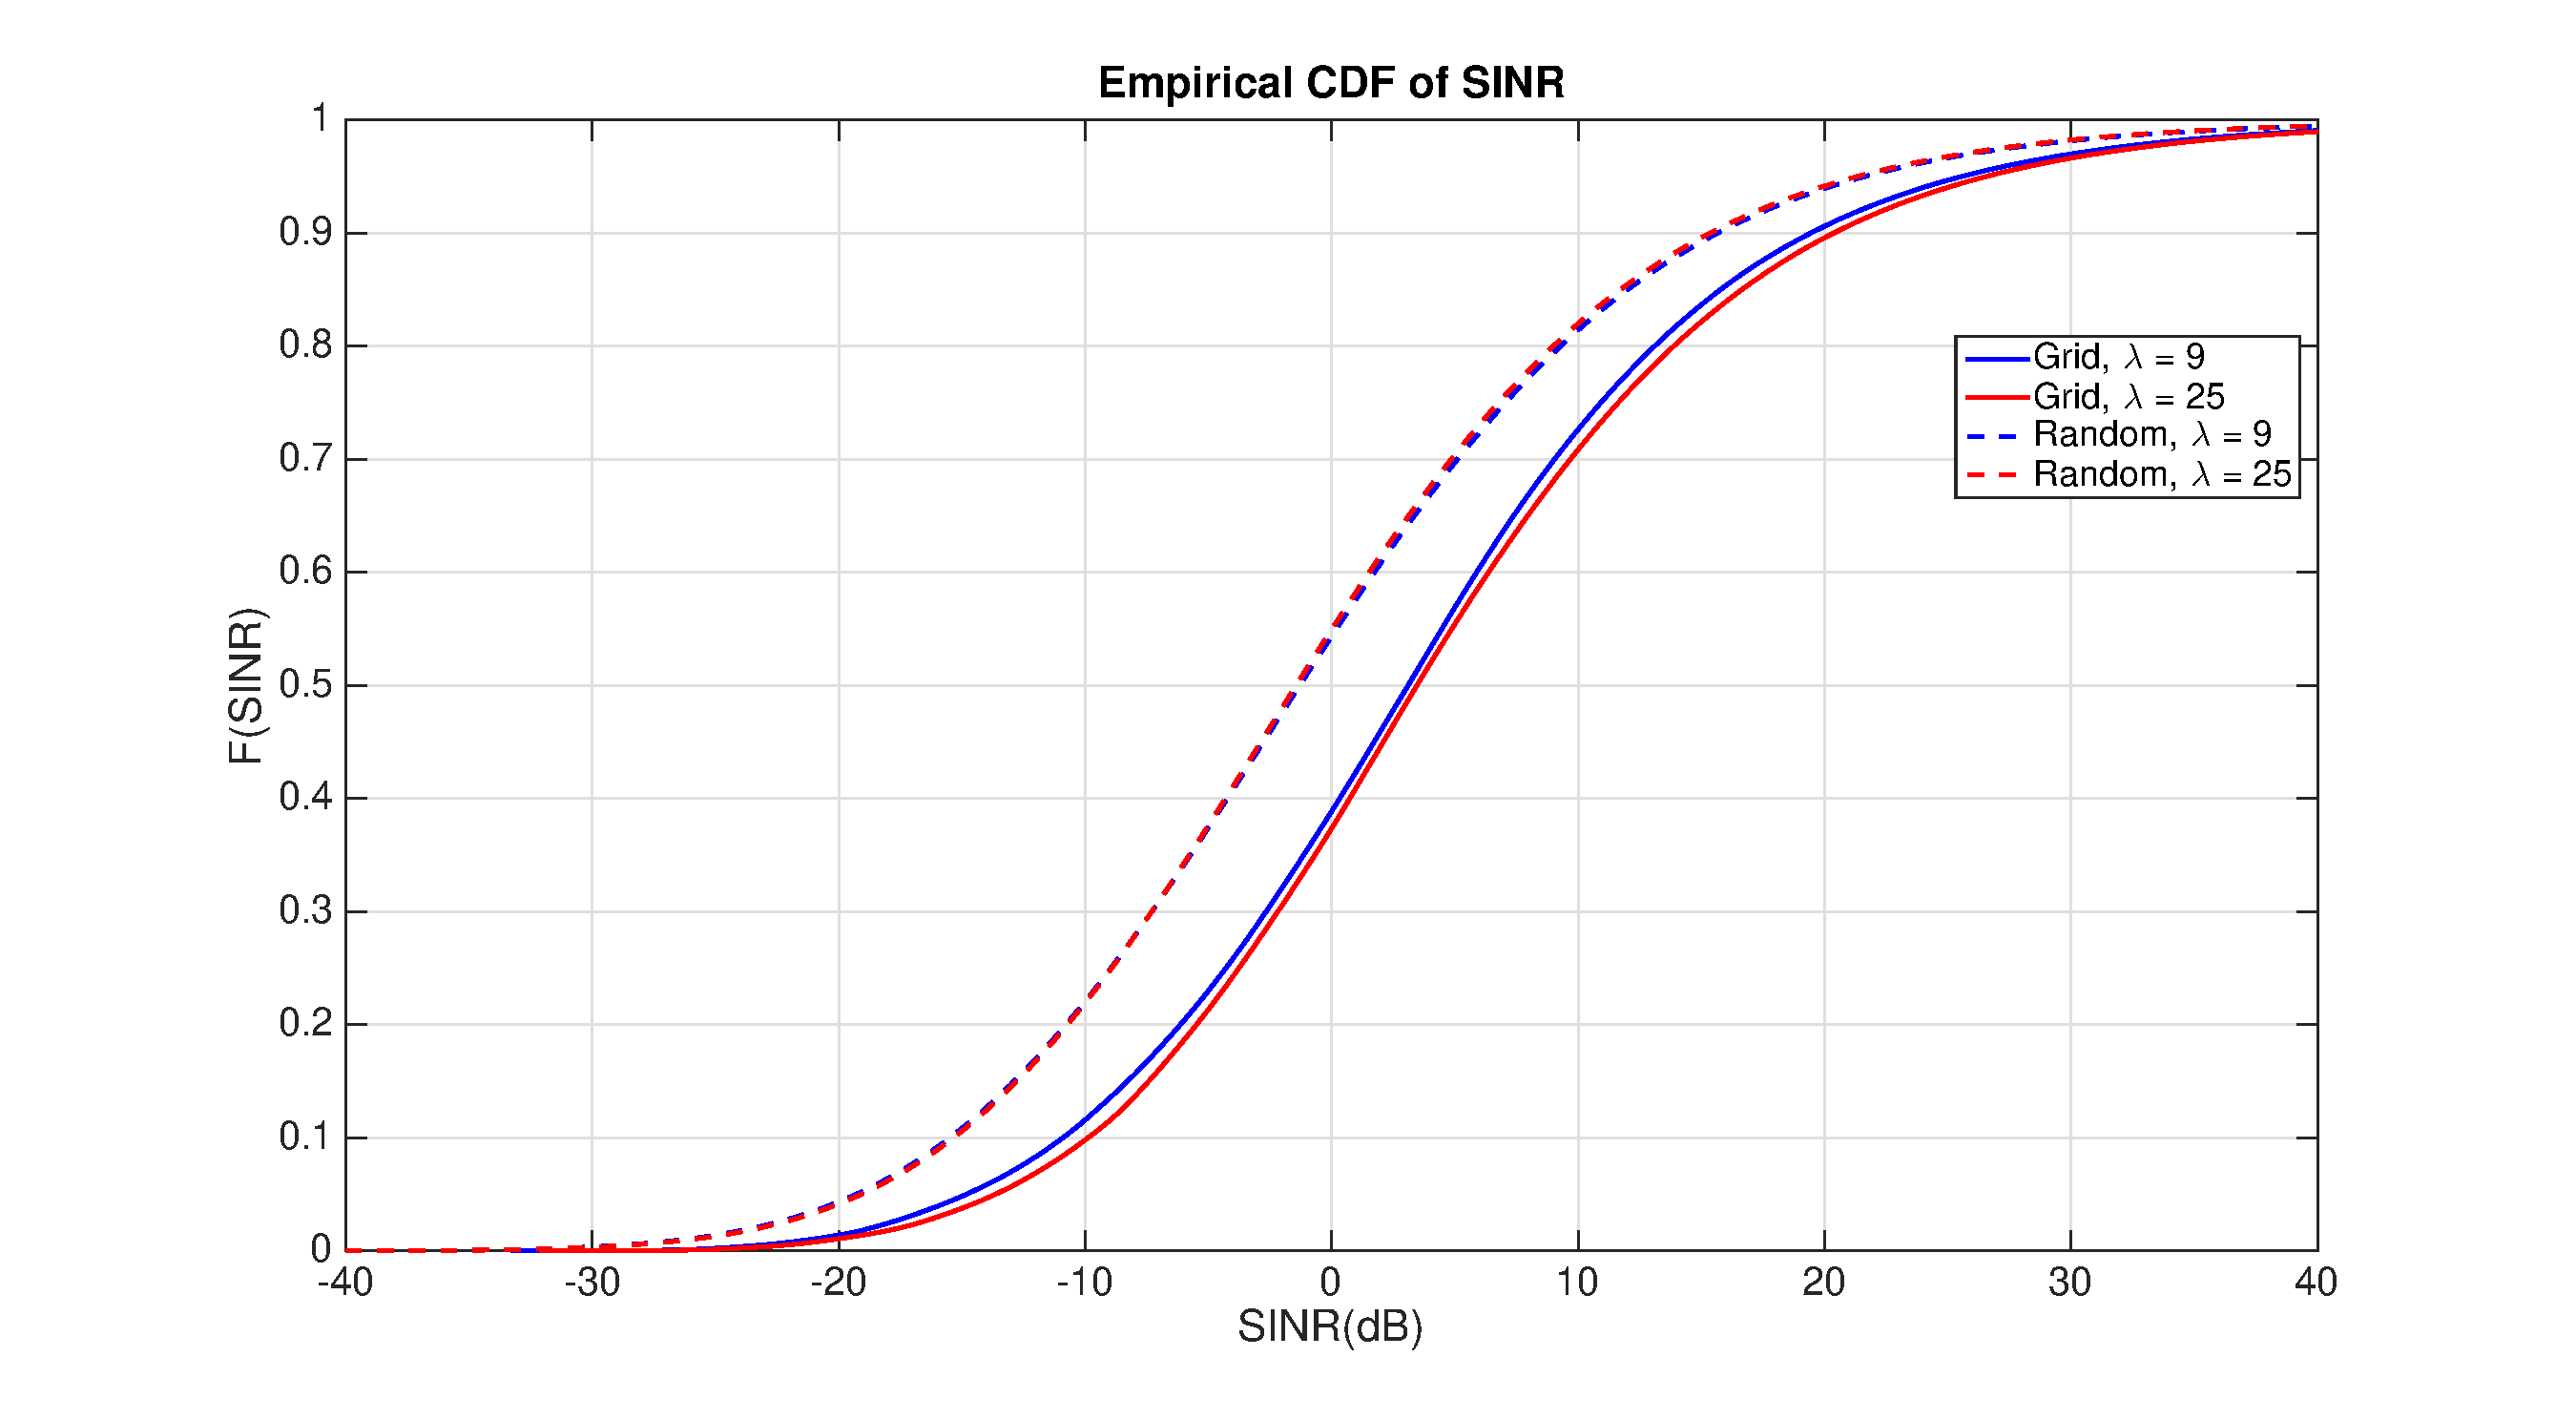
\includegraphics[width=6cm]{GridVSRandom.eps}
 \caption{CDF of SINR given Grid model and Random model (de-correlation distance: $20m$)}
 \label{4:cdf1}
 \end{figure}
 \column{.5\textwidth}
 \begin{figure}
 \centering
 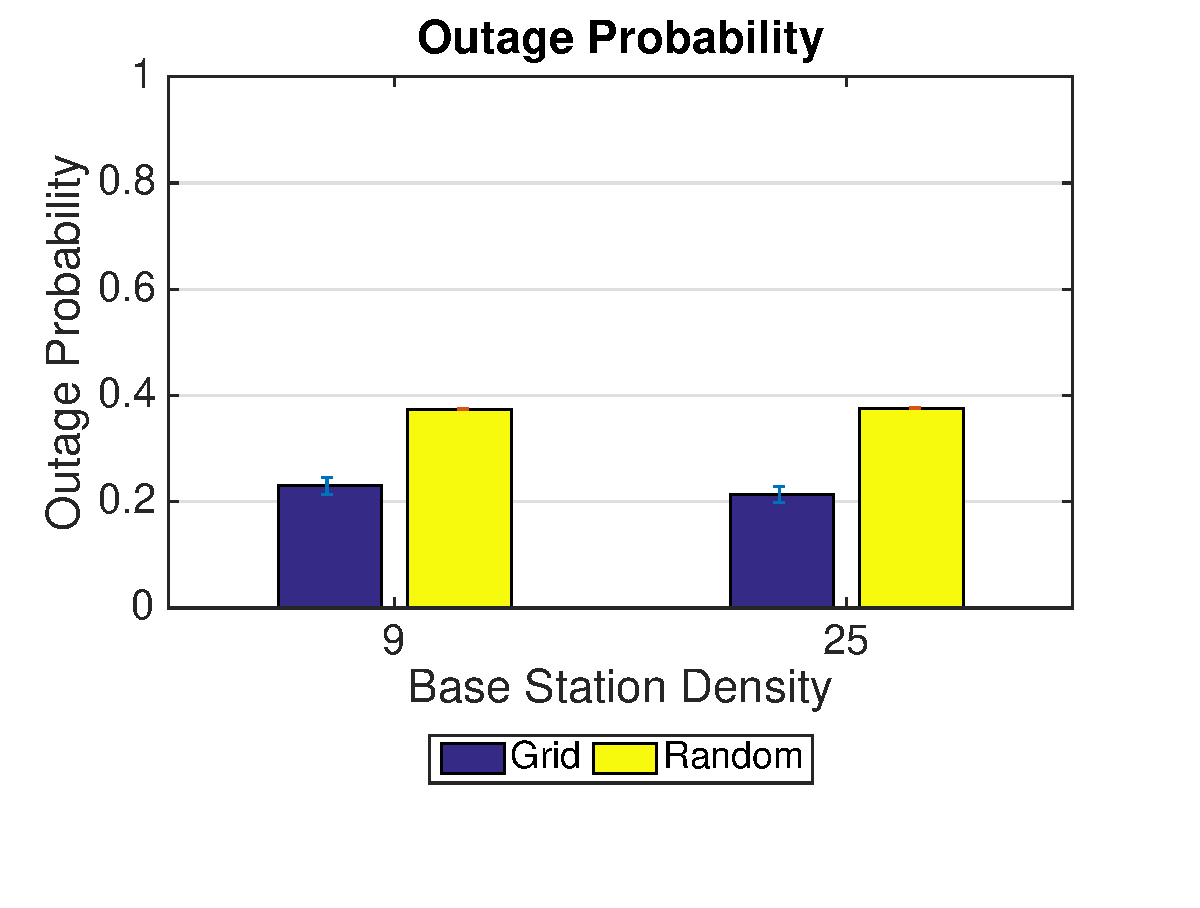
\includegraphics[width=6cm]{OutageProbGridVSRandom.eps}
 \caption{Outage probability given Grid model and Random model with $\gamma = -5dB$ (de-correlation distance: $20m$)}
 \label{4:outage1}
 \end{figure}
 \end{columns}
\end{frame}
\begin{frame}
\subsection{Outage Probability and Outage Durations}
\frametitle{Outage Probability Simulation}
\begin{table}
 \centering
 \caption{\label{SystemConfig2}Simulation Configuration Parameters}

 \begin{tabular}{|c|c|}

 \hline
 Target Area & $1000m\times 1000m$\\
 \hline
 BS Densities & $3, 10, 50, 100, 200, 300, 500$\\
 \hline
 Path Loss Exponent & $4$\\
 \hline
 BS Transmission Power & $P: 40dbm$\\
 \hline
 SINR Requirement & $-5dB$\\
 \hline
 De-Correlation Distance & $20m, 200m$\\
 \hline
 \end{tabular}

 \end{table}
\end{frame}

\begin{frame}
\frametitle{Outage Probability Analysis}
\begin{columns}[c]
\column{.5\textwidth}
 \begin{figure}
 \centering
 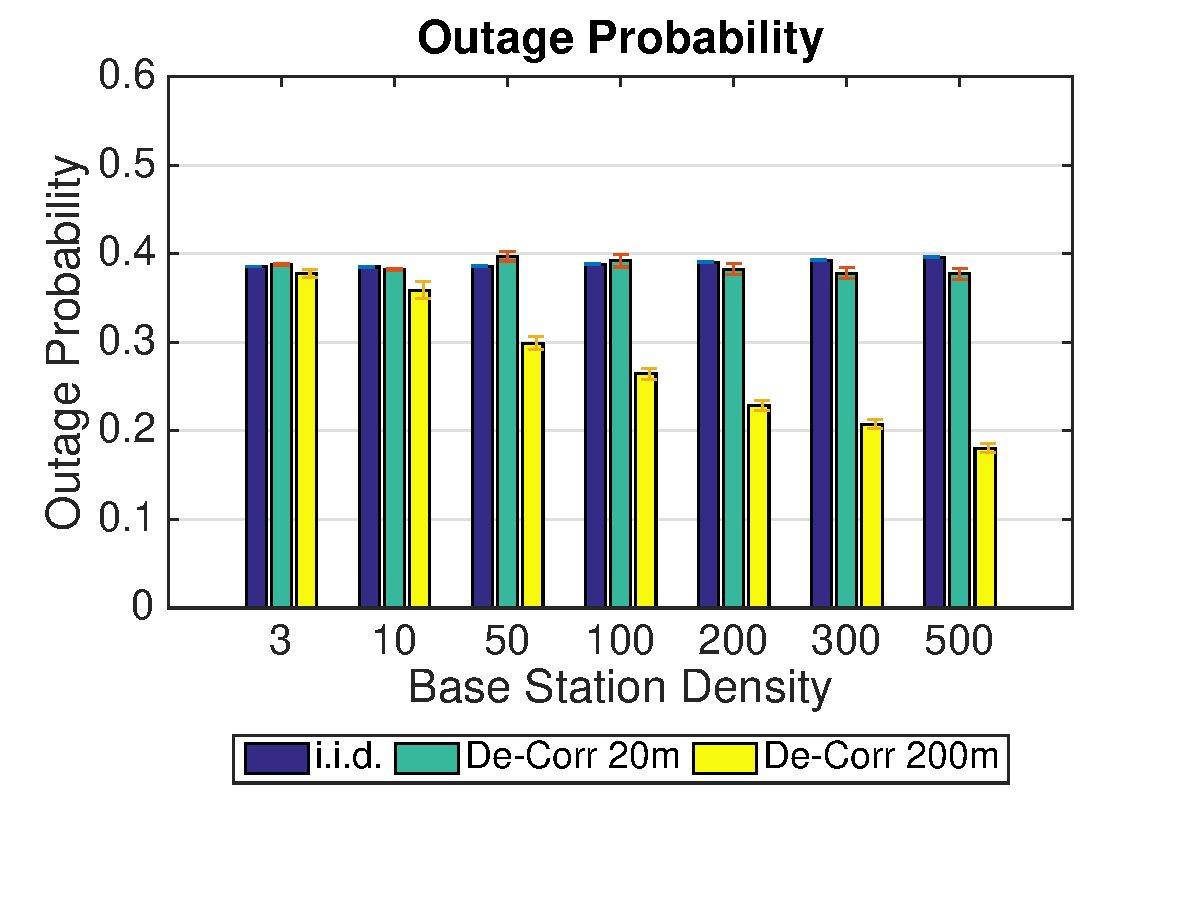
\includegraphics[width=6cm]{NBMax1000OutageProbThresh-5iid.eps}
 \caption{Outage probability given $-5dB$ SINR threshold (MS connecting to the Nearest BS)}
 \label{fig: outprob1}
 \end{figure}
 \column{.5\textwidth}
 \begin{figure}
 \centering
 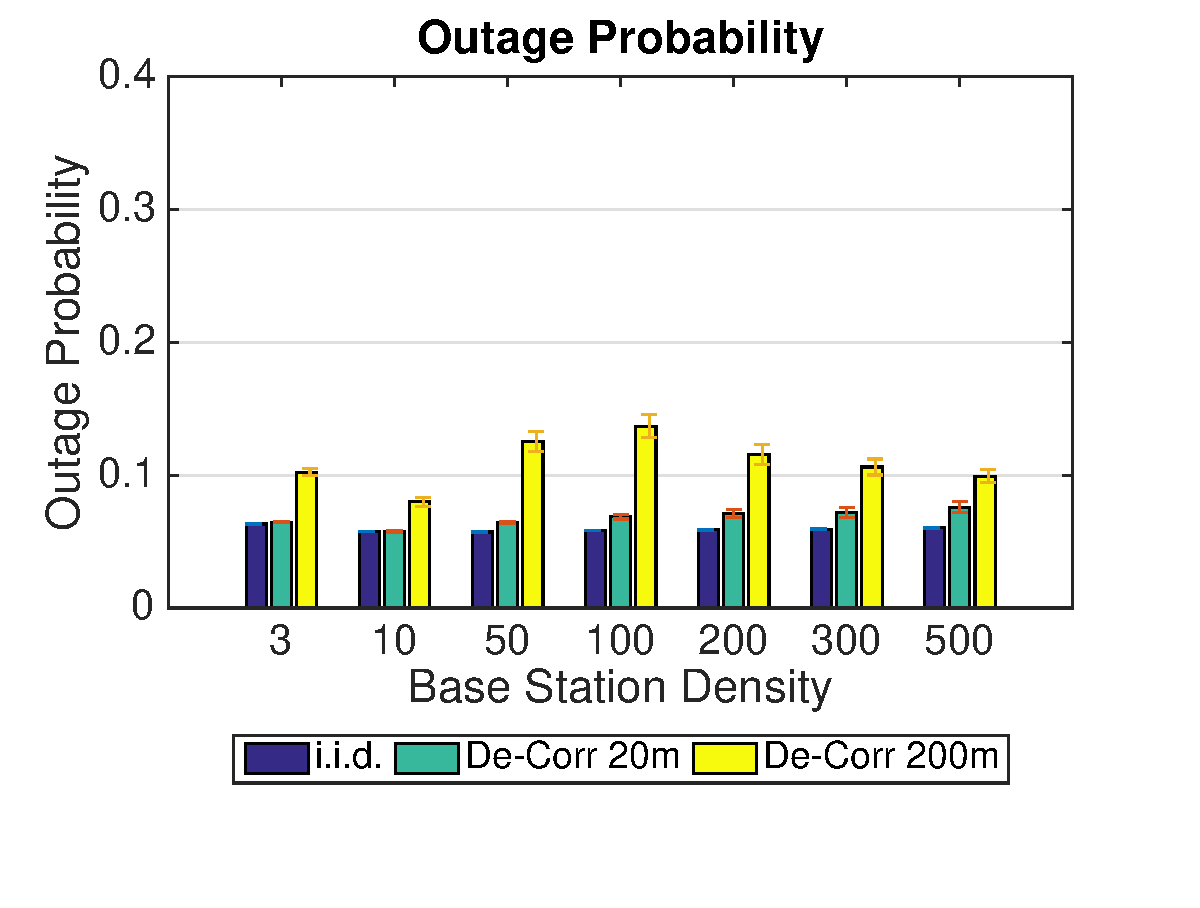
\includegraphics[width=6cm]{MaxMax1000OutageProbThresh-5iid.eps}
 \caption{Outage probability given $-5dB$ SINR threshold (MS connecting to the Strongest BS)}
 \label{fig: outprobs2}
 \end{figure}
  \end{columns}
\end{frame}

\begin{frame}
\frametitle{Outage Duration Analysis}
\begin{columns}[c]
\column{.5\textwidth}
 \begin{figure}
 \centering
 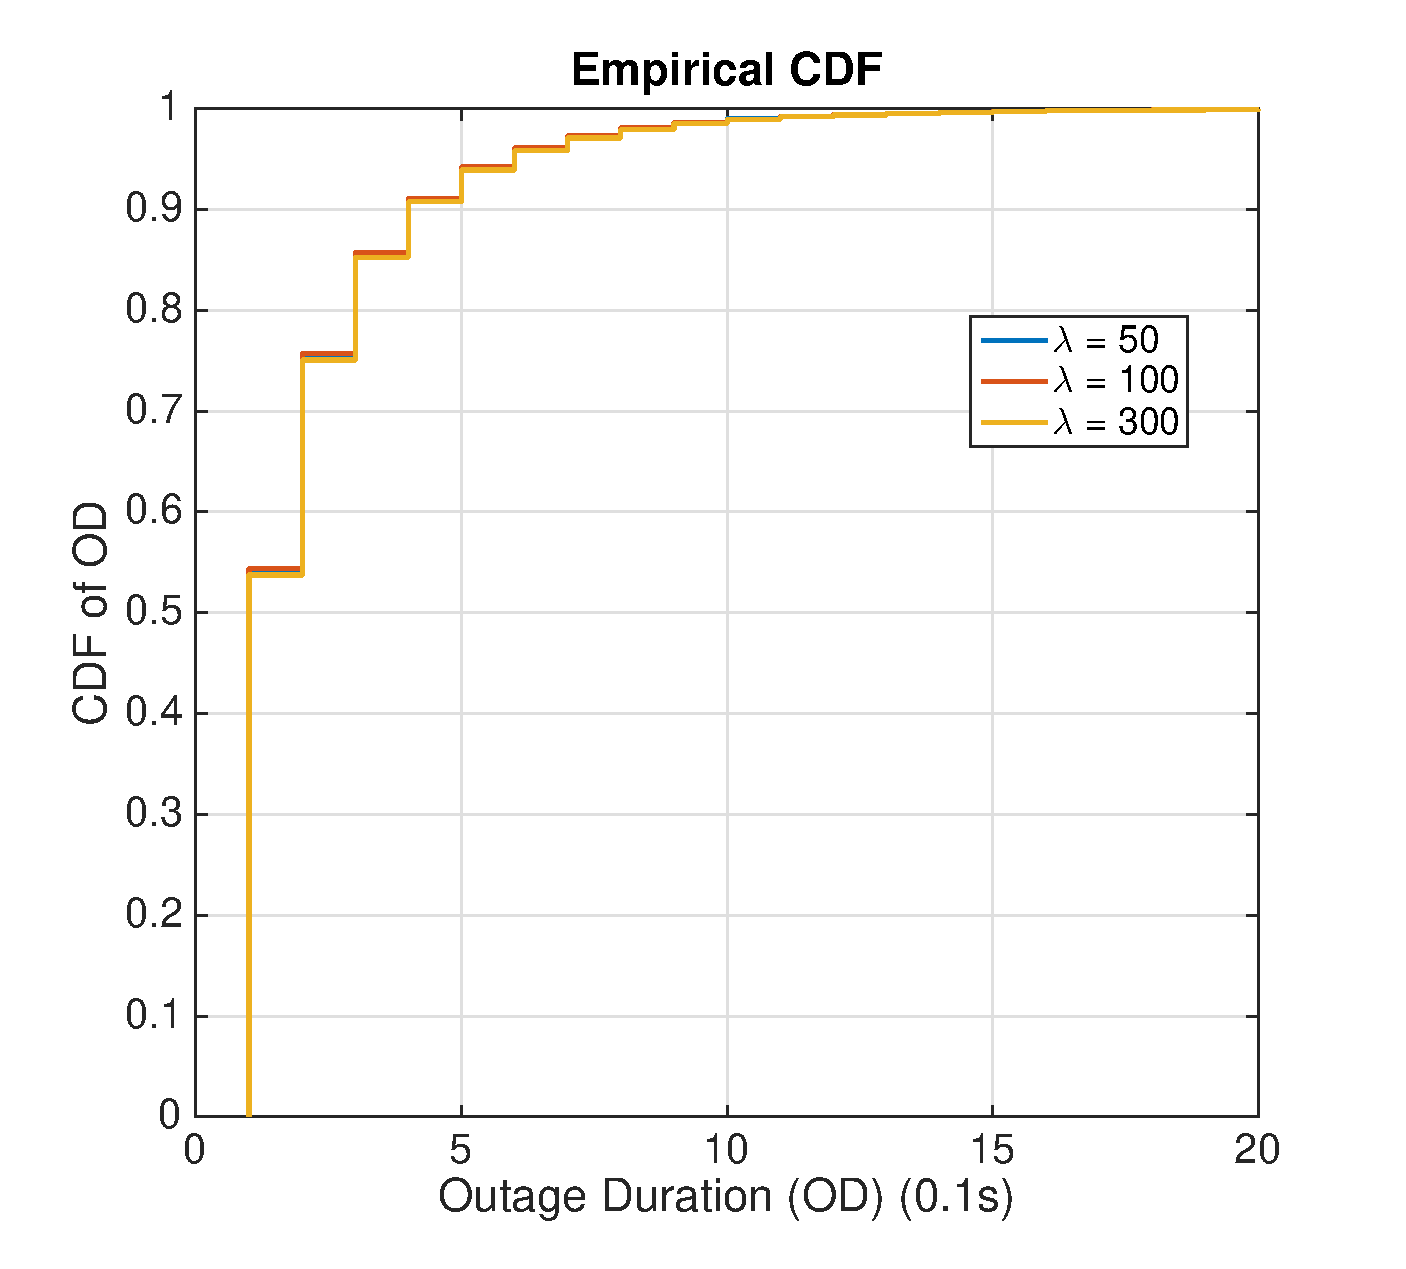
\includegraphics[width=5cm]{ODthresh-5iidNB.eps}
 \caption{CDF of Outage Durations when the MS is connecting to the Nearest BS with independent shadow fading}
 \label{iid1}
 \end{figure}
 \column{.5\textwidth}
 \begin{figure}
 \centering
 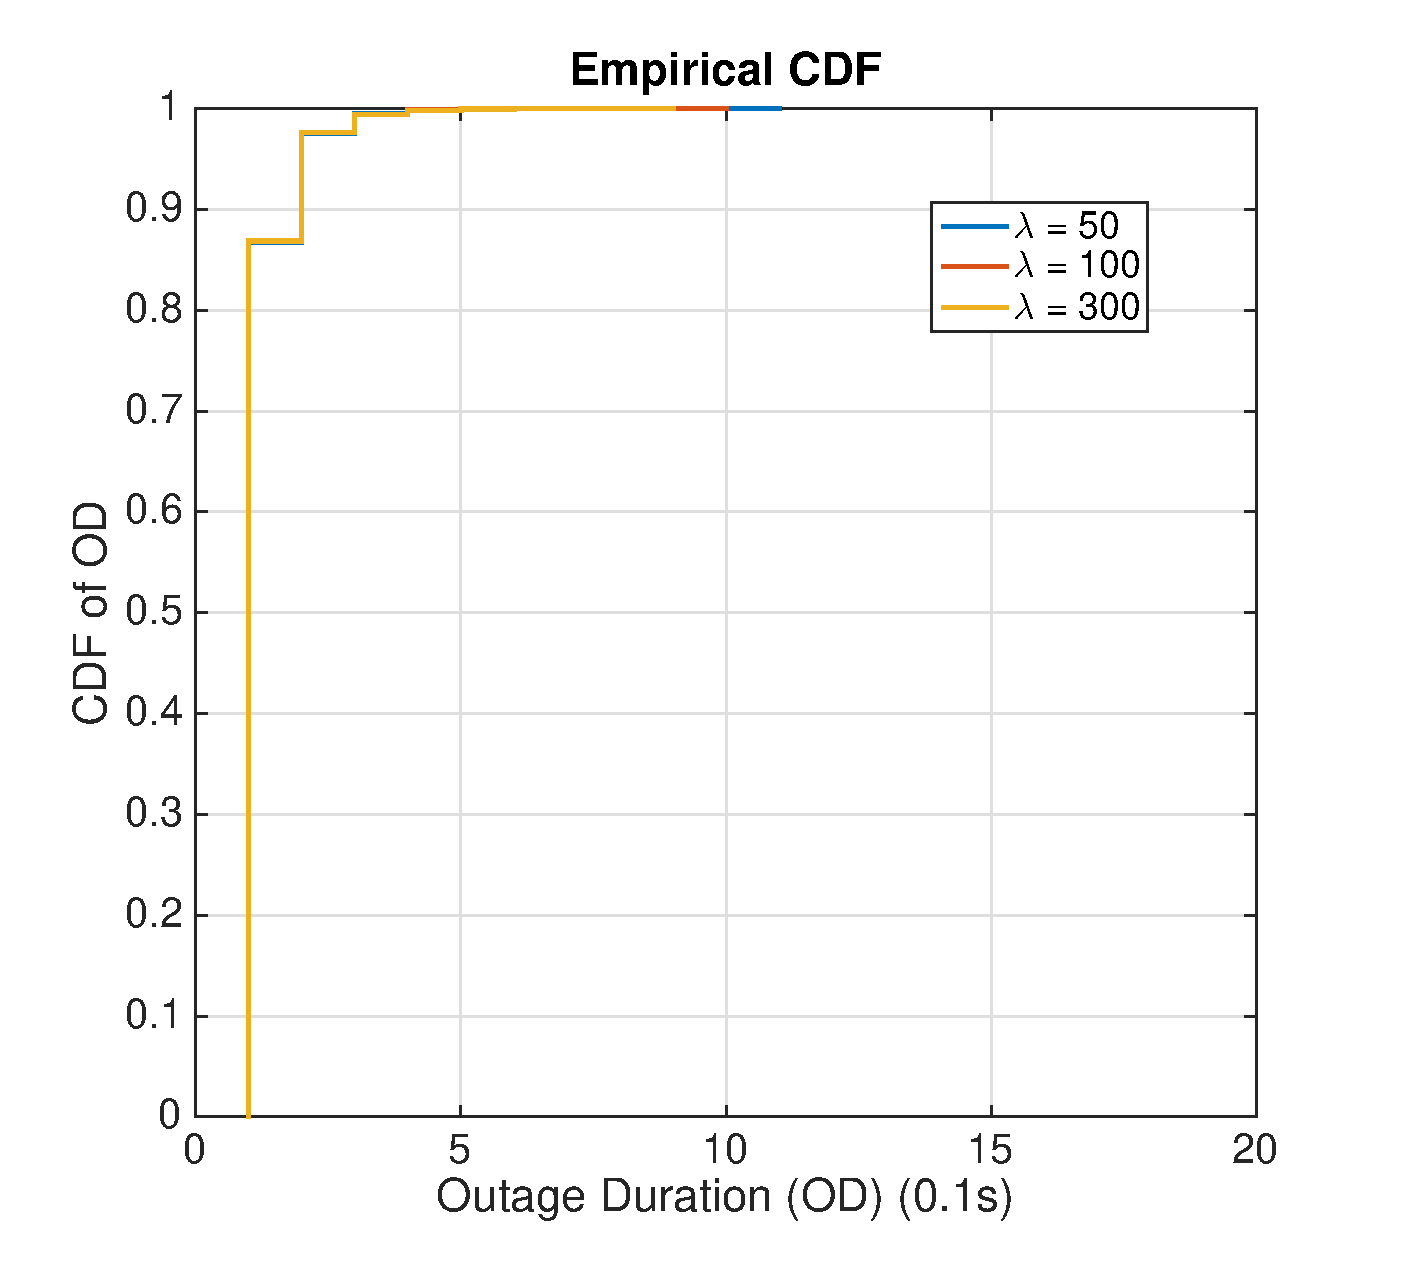
\includegraphics[width=5cm]{ODthresh-5iidMax.eps}
 \caption{CDF of Outage Durations when the MS is connecting to the Strongest BS with independent shadow shadowing}
 \label{iid2}
 \end{figure}
 \end{columns}
 \end{frame}
 \begin{frame}
 \frametitle{Outage Duration Analysis Cont'd}
 \begin{columns}[c]
 \column{.5\textwidth}
 \begin{figure}
 \centering
 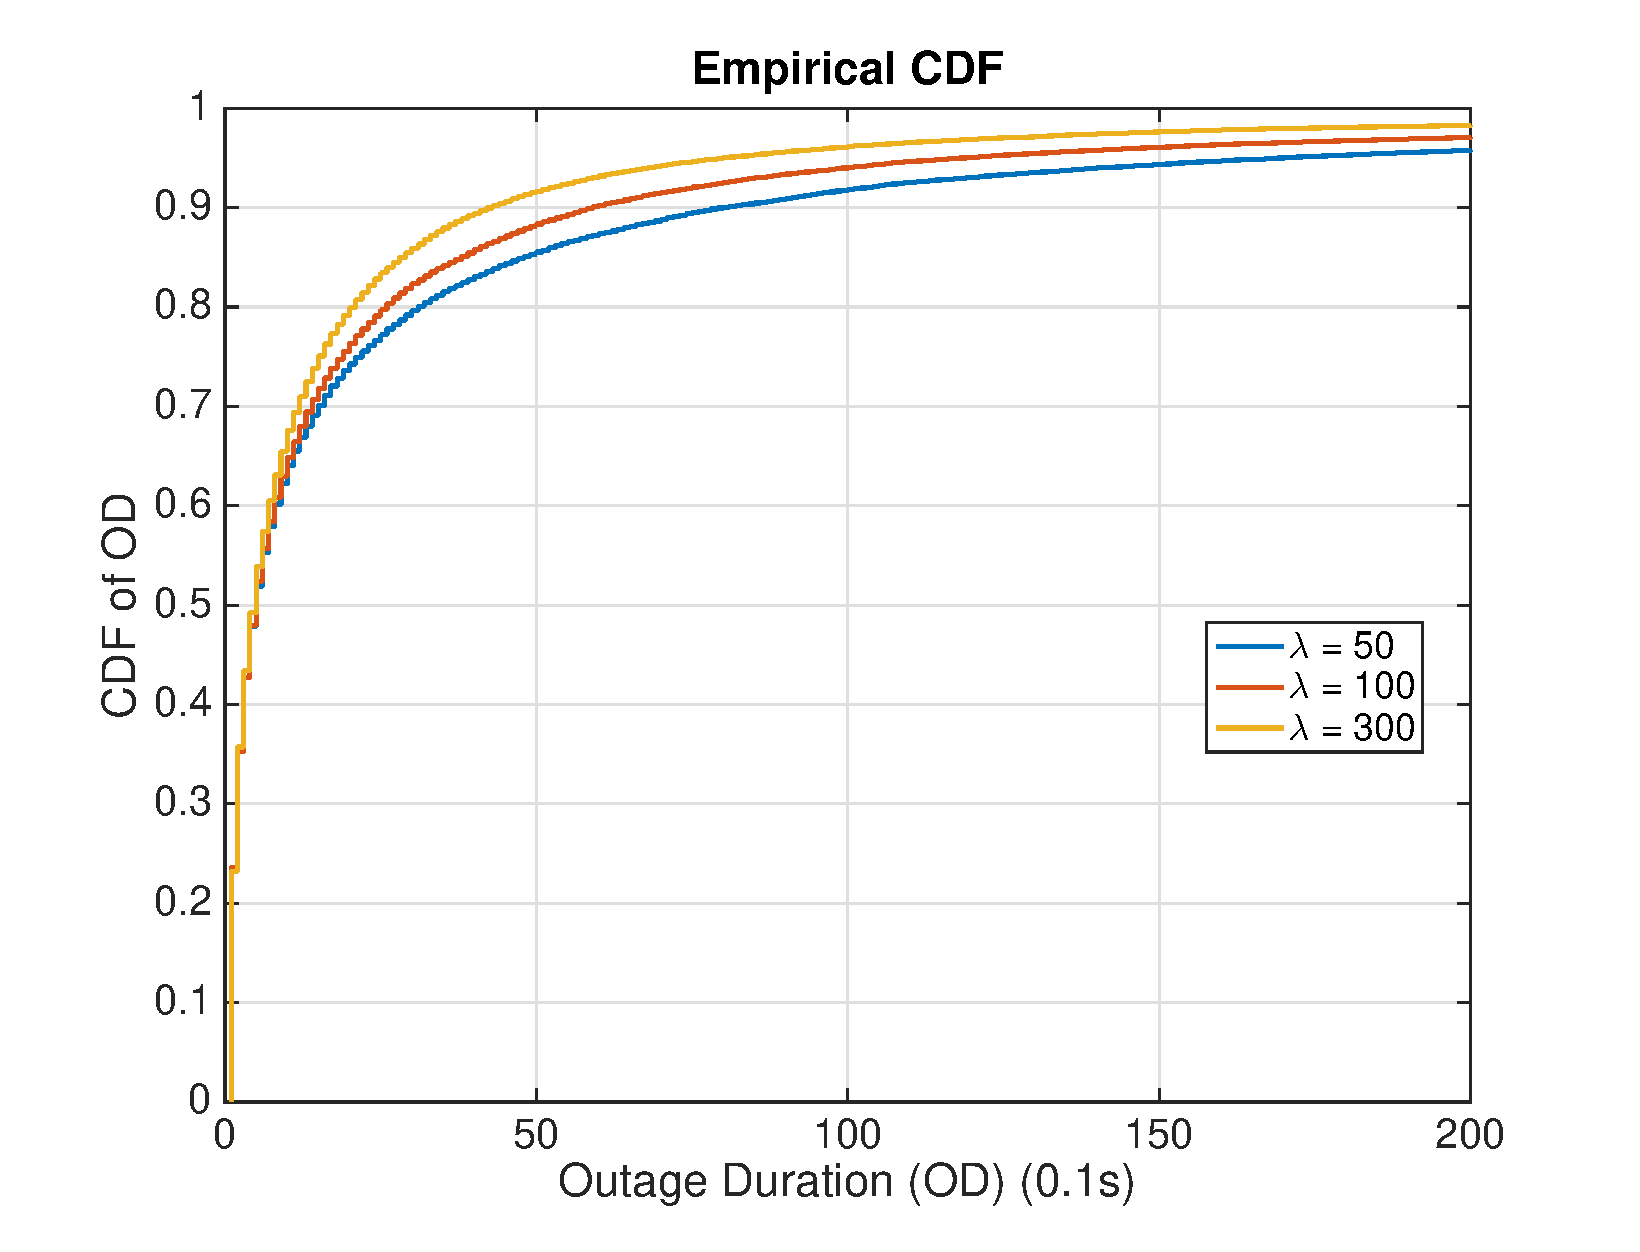
\includegraphics[width=5cm]{ODthresh-5DeCorr200NBMode2.eps}
 \caption{CDF of Outage Durations when MS is connecting to the Nearest BS with correlated shadowing (de-correlation distance: 200m)}
 \label{corr1}
 \end{figure}
  \column{.5\textwidth}
 \begin{figure}
 \centering
 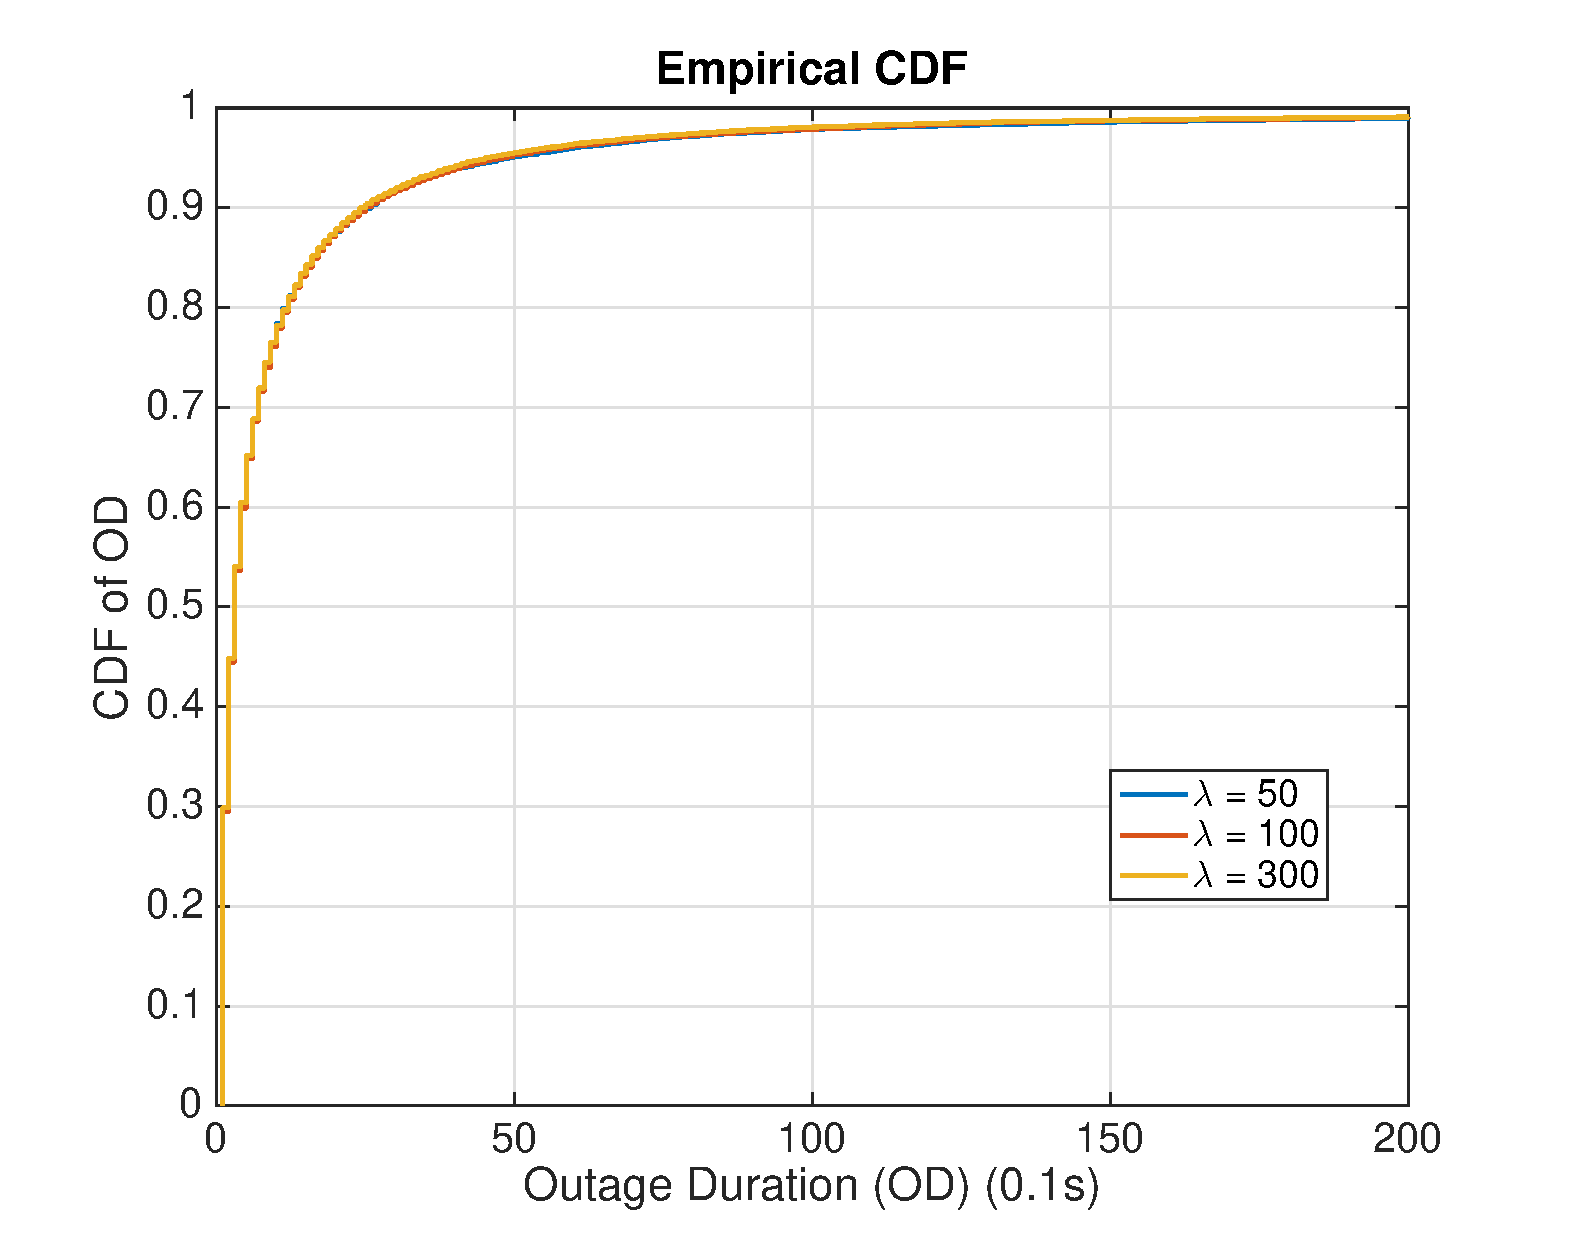
\includegraphics[width=5cm]{ODthresh-5DeCorr200MaxMode2.eps}
 \caption{CDF of Outage Durations when MS is connecting to the Strongest BS with correlated shadowing (de-correlation distance: 200m)}
 \label{corr2}
 \end{figure}
 \end{columns}
\end{frame}
\section{Transport Layer Protocols for Next Generation Networks}
\subsection{Motivation}
\begin{frame}
\frametitle{Motivation}
MmWave Channel:
\begin{itemize} 
\item High capacity and low delay.
\item Sensitive to obstructions, which result in frequent capacity fluctuations.
\item Switch between line-of-sight (LOS) state and none-line-of-sight (NLOS) state periodically.
\end{itemize}
\begin{block}{Legacy TCP}
Legacy TCP congestion control protocols might not work well with mmWave channel due to the slow congestion detection and conservative loss recovery.
\end{block}
\end{frame}
\begin{frame}
\frametitle{Test Legacy TCP on an Emulated MmWave Channel}
\begin{figure}
\centering
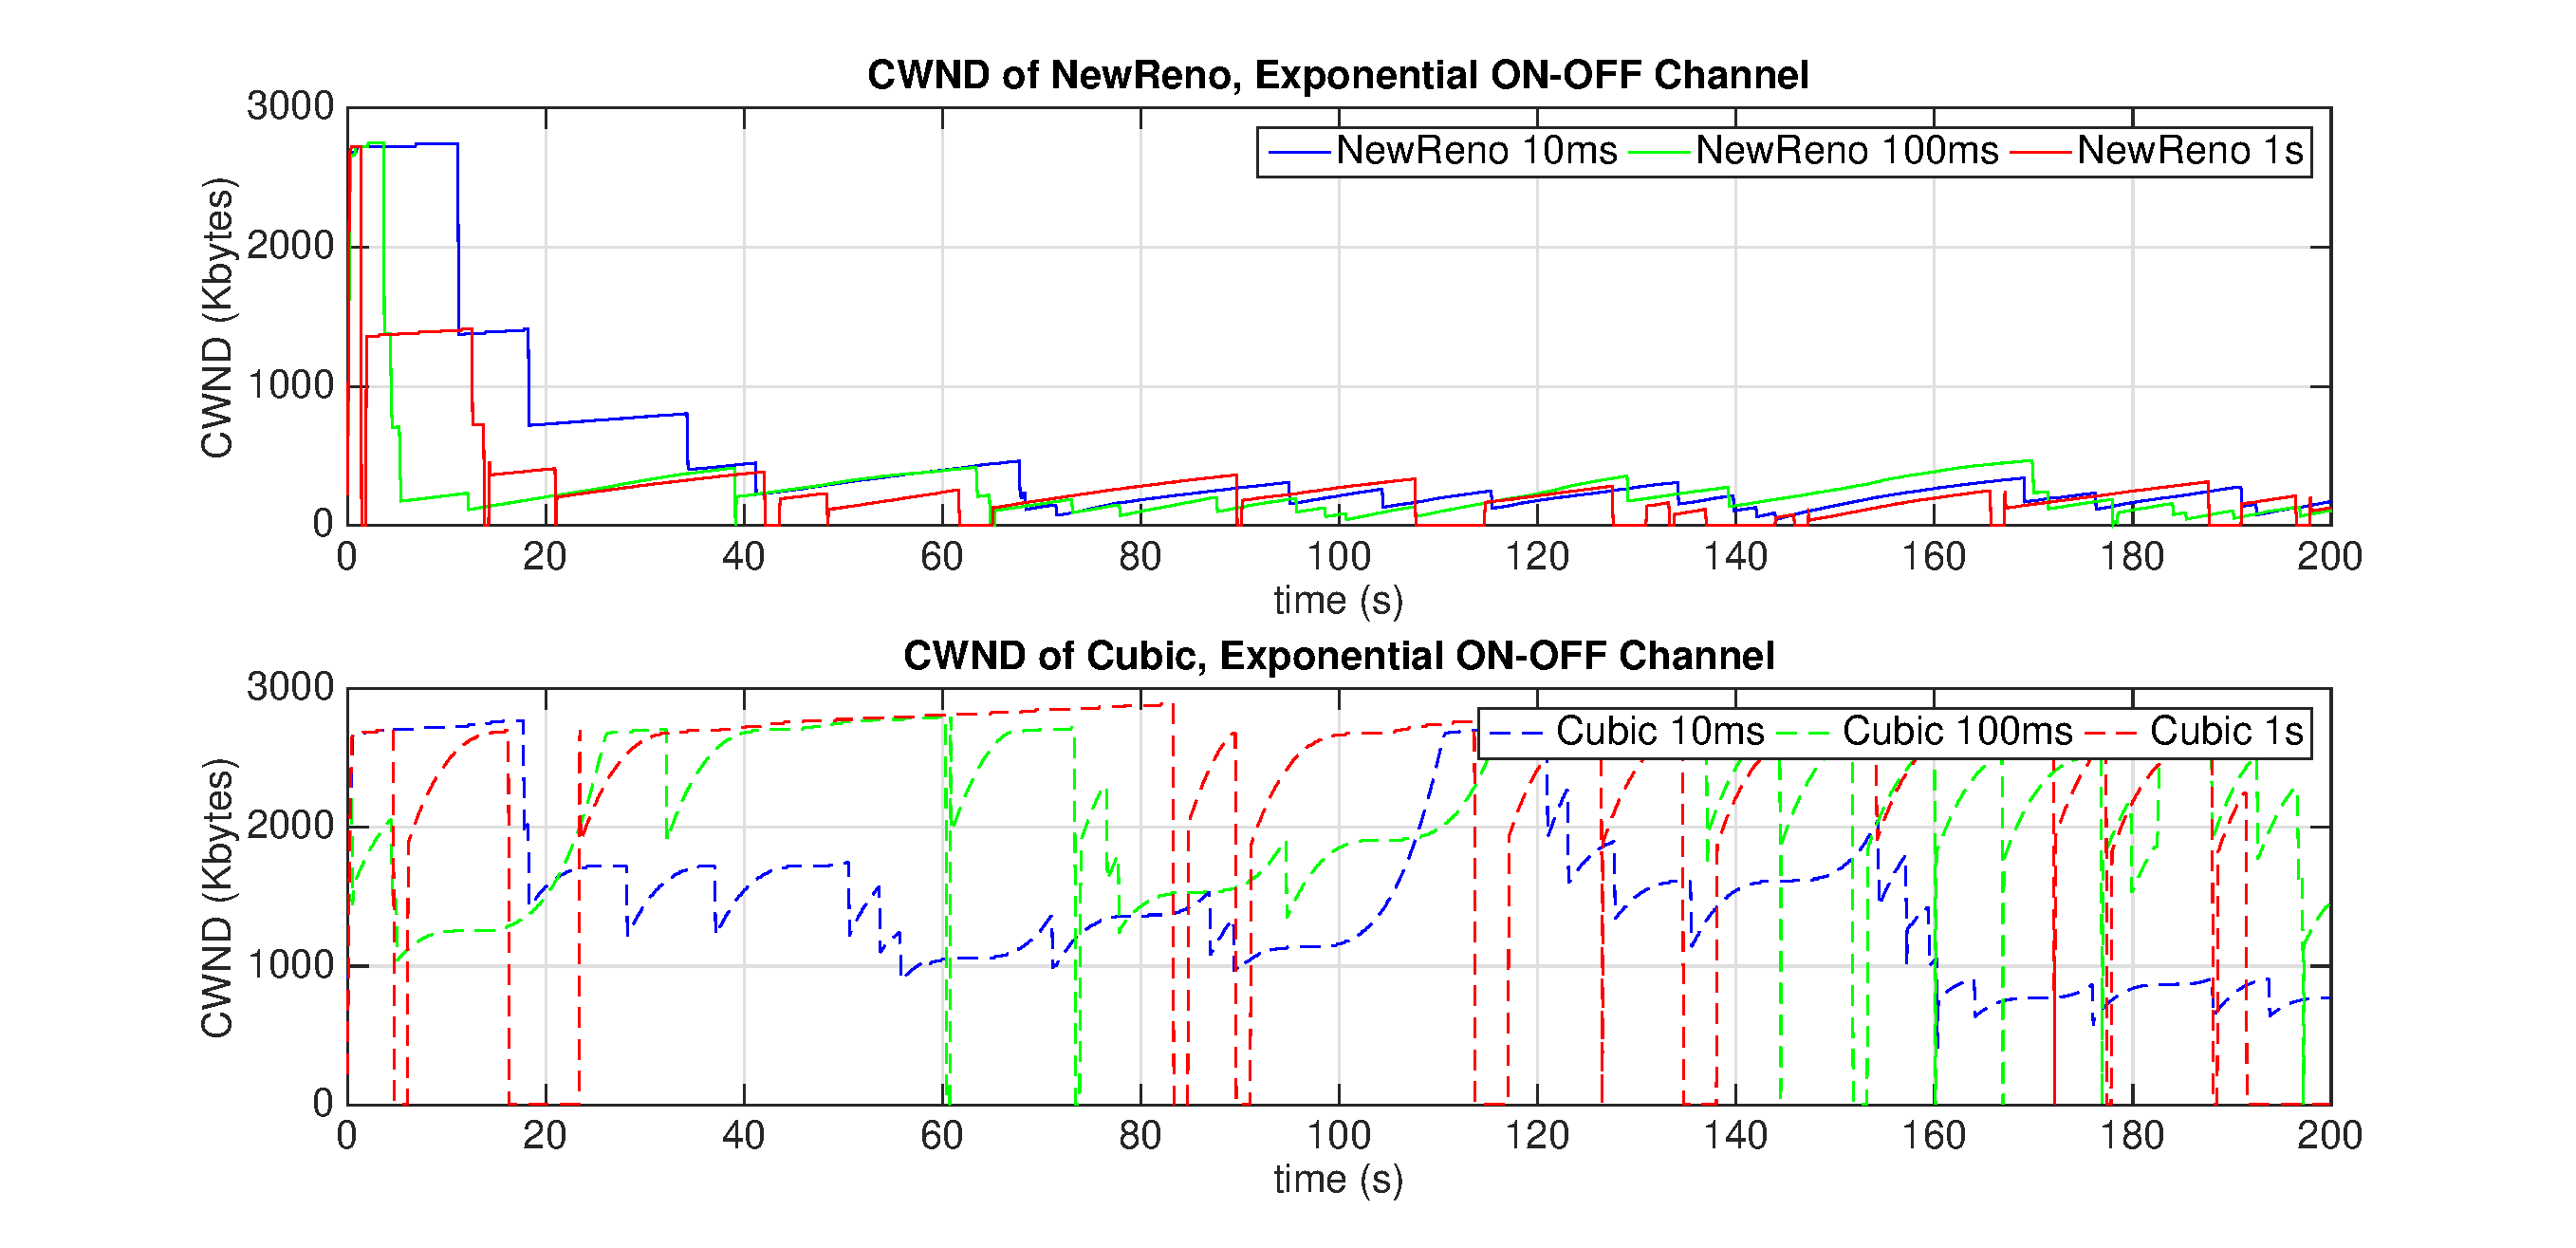
\includegraphics[width=10cm]{1.eps}
\caption{CWND dynamics given exponentially On-Off channel behavior}
\label{1st}
\end{figure}
\end{frame}
%\begin{figure}
%\centering
%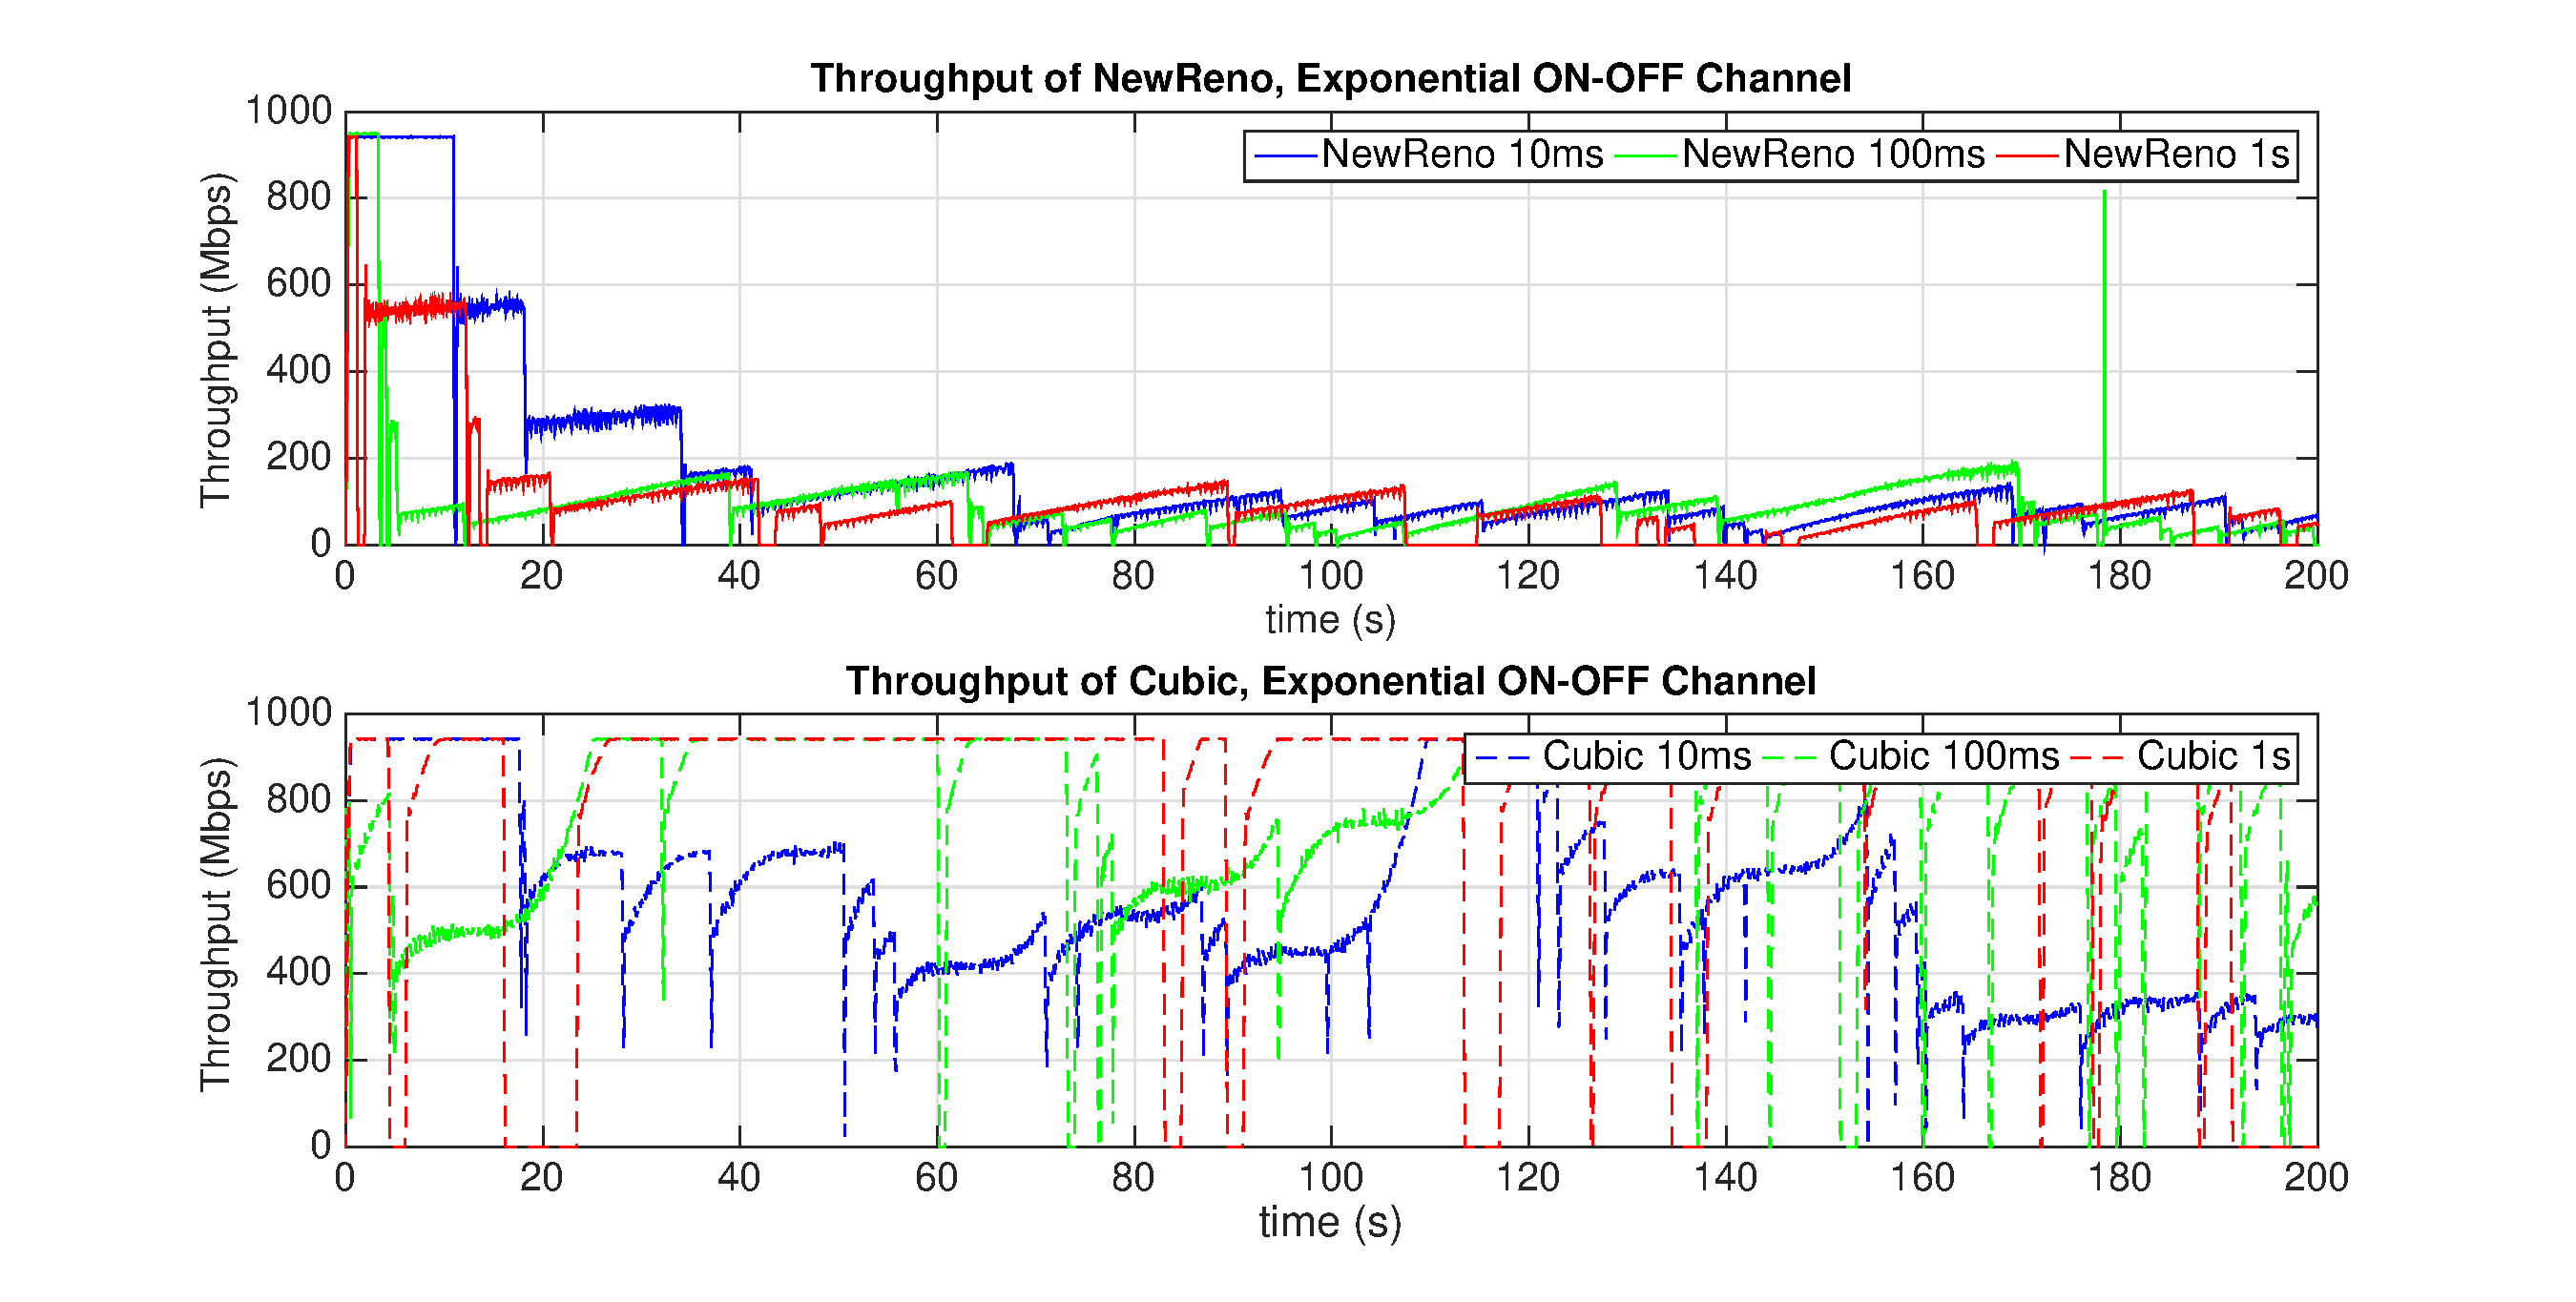
\includegraphics[width=10cm]{2.eps}
%\caption{Throughput dynamics given exponentially On-Off channel behavior}
%\label{2nd}
%\end{figure}
\begin{frame}
\frametitle{Test Legacy TCP on an Emulated MmWave Channel Cont'd}
\begin{figure}
\centering
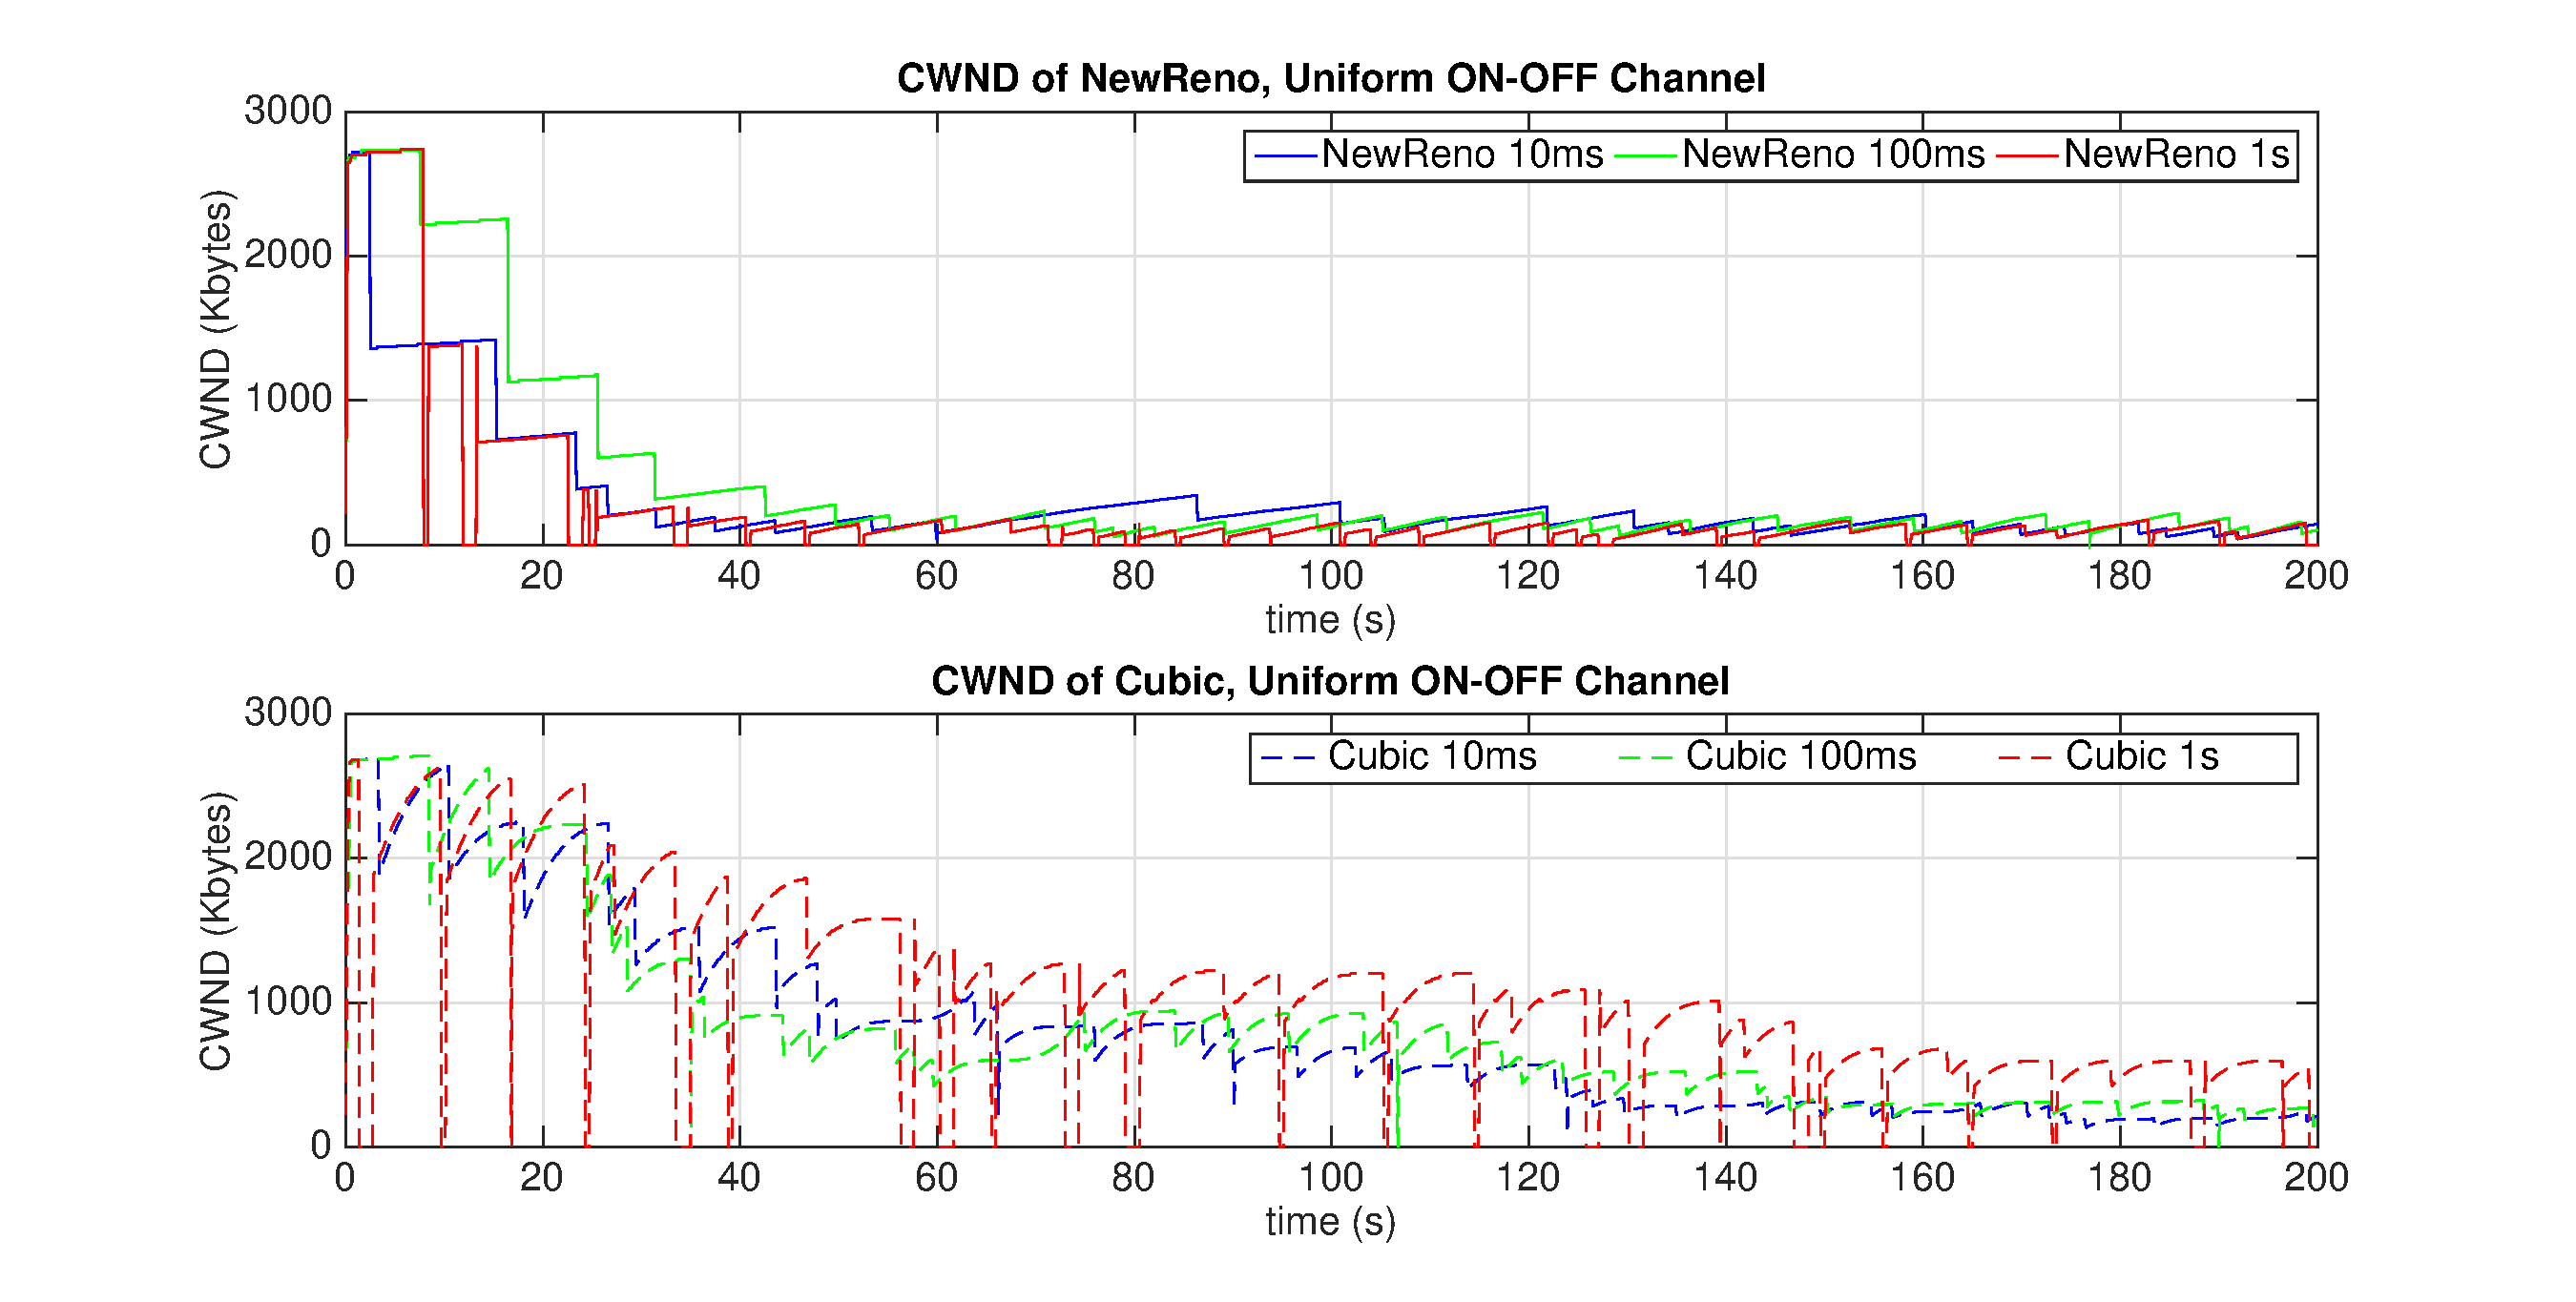
\includegraphics[width=10cm]{3.eps}
\caption{CWND dynamics given uniformly On-Off channel behavior}
\label{3rd}
\end{figure}
%\begin{figure}
%\centering
%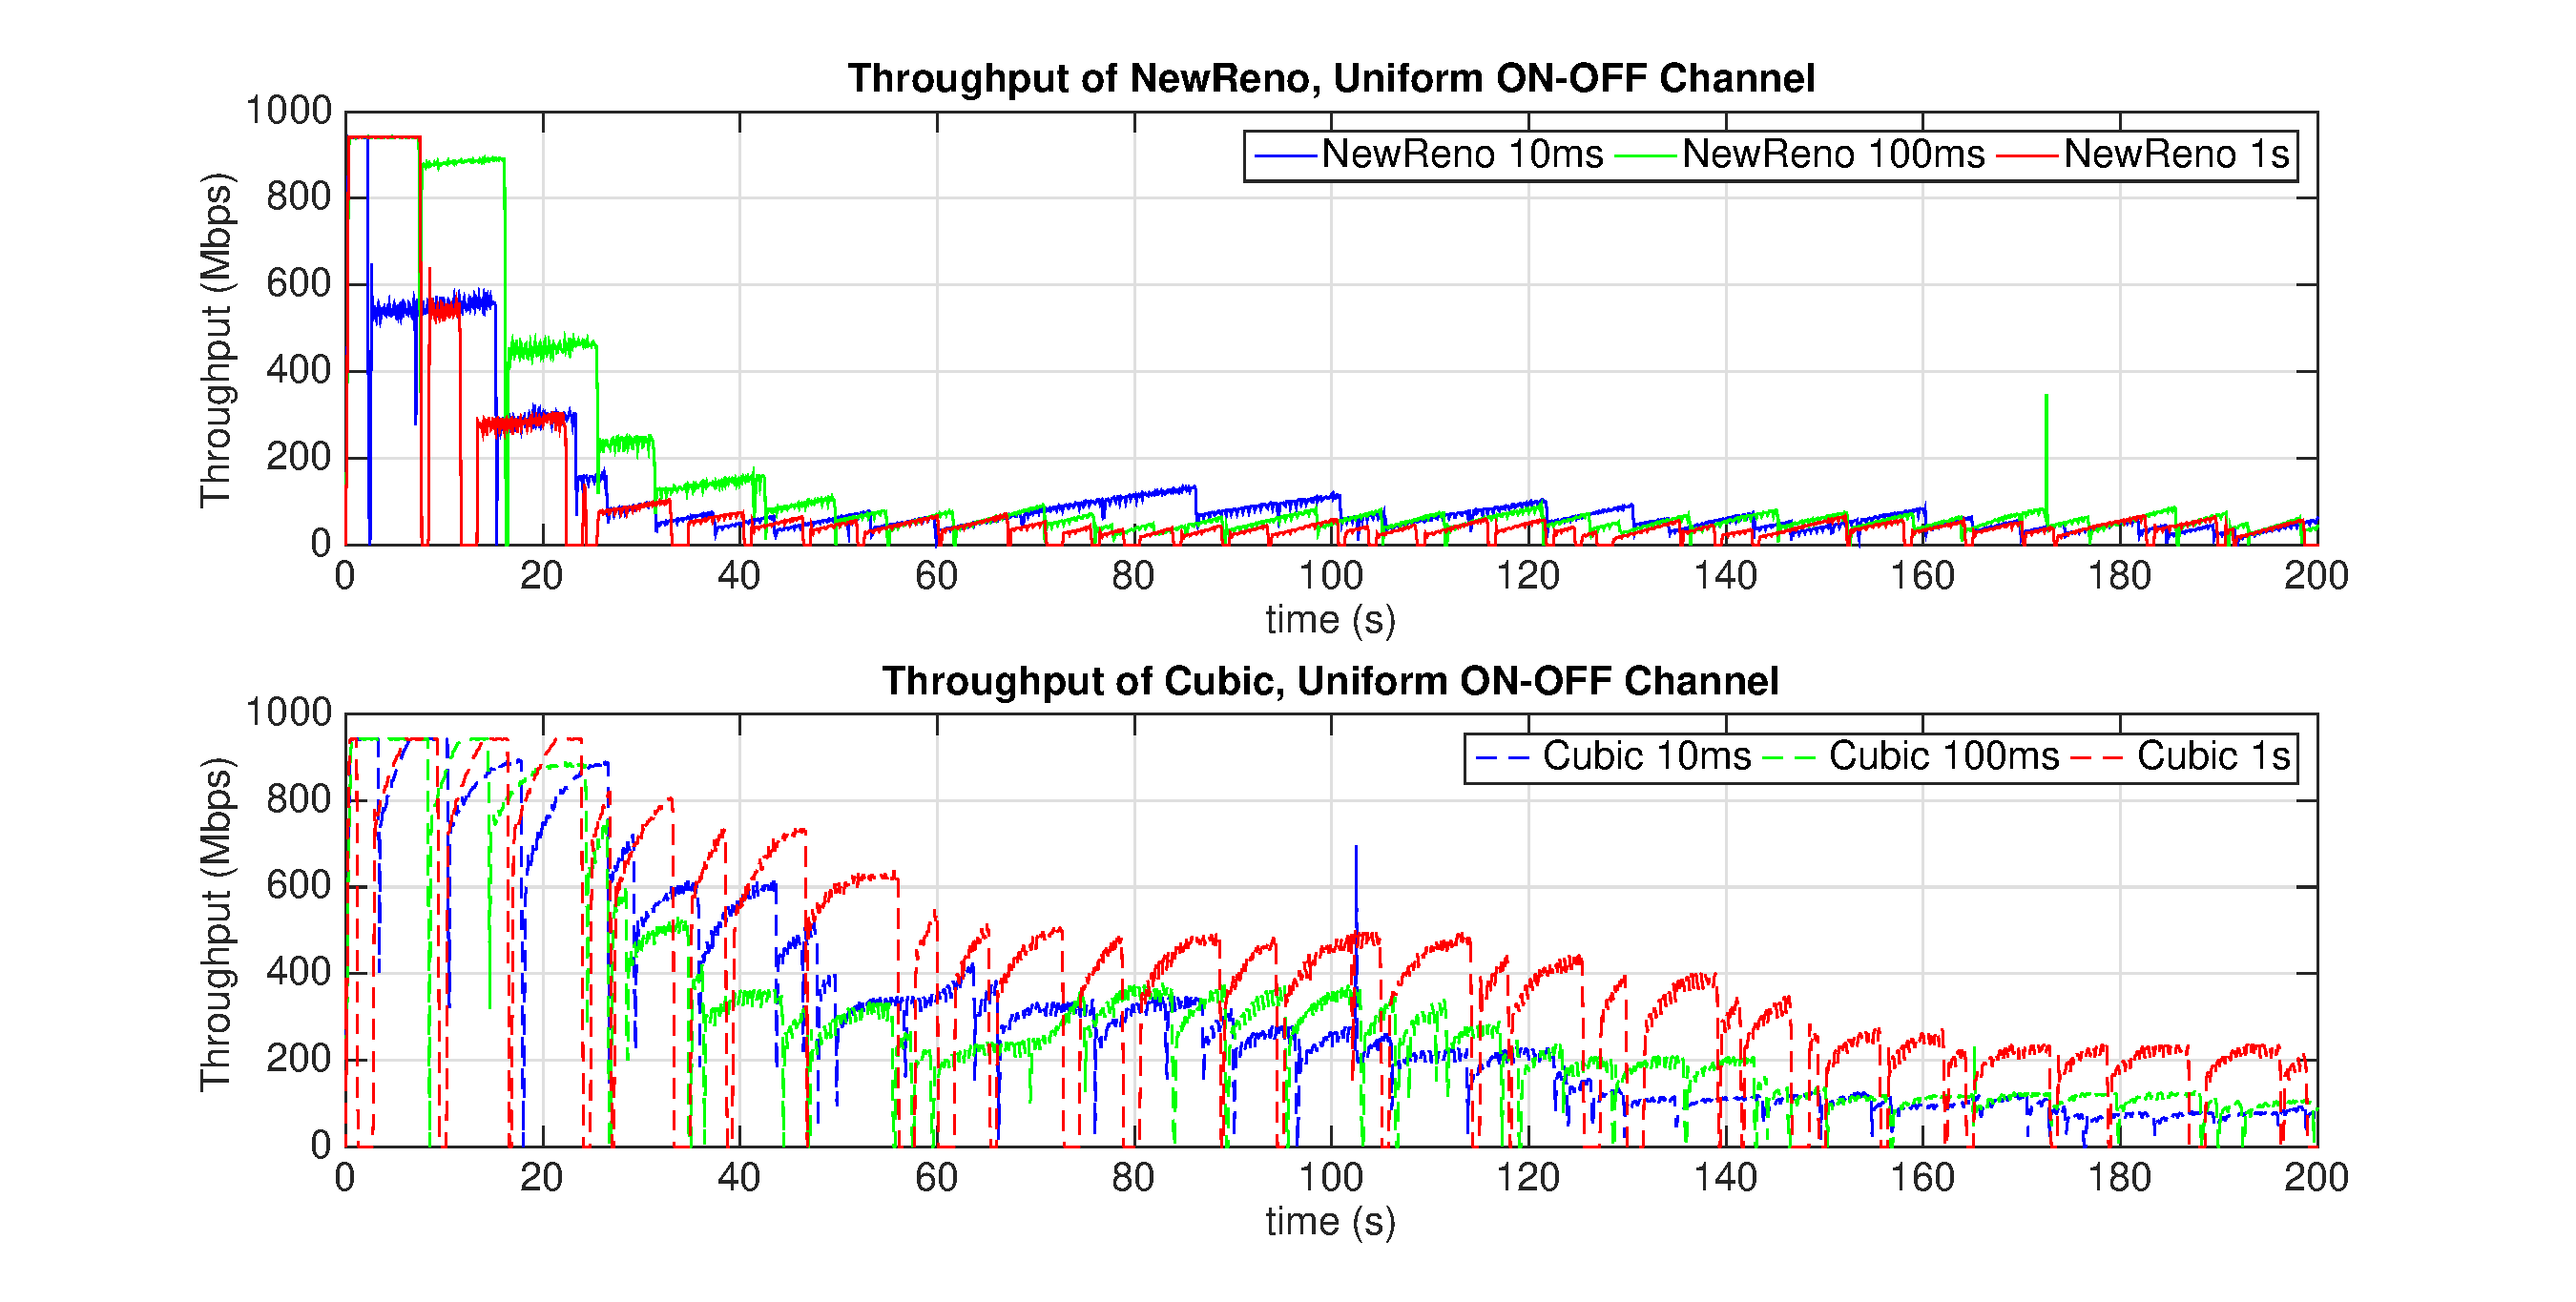
\includegraphics[width=10cm]{4.eps}
%\caption{Throughput dynamics given uniformly On-Off channel behavior}
%\label{4th}
%\end{figure}

\end{frame}
%\subsection{Remy and Explicit Congestion Notification (ECN)}
\begin{frame}
\frametitle{Remy}
Remy is a congestion-control scheme based on prior knowledge of the network and the traffic model. It is the first computer generated congestion control protocol. A RemyCC tracks only three state variables of the end-user:
\begin{itemize}
\item An exponentially weighted moving average (EWMA) of the inter-arrival time between new ACKs received (ack\_ewma).
\item An EWMA of the time between TCP sender timestamps reflected in those ACKs (send\_ewma).
\item The ratio between the most recent Round Trip Time (RTT) and the minimum RTT during the current connection (rtt\_ratio).
\end{itemize}
This algorithm does not require the support from any intermediate network devices. The end-user can adjust its sending speed following the pre-generated algorithm based on the above data.
\end{frame}

\begin{frame}
\frametitle{Explicit Congestion Notification (ECN)}
With the addition of active queue management and ECN to the network infrastructure, routers are capable of detecting congestion before queue overflows. 
\begin{itemize}
\item An additional Congestion Experienced (CE) byte is added to the IP header of the packet to support this function.
\item Routers running RED queue management can mark the CE code point with a certain probability when the average queue length satisfies a certain criteria.
\item The packet with marked CE will be sent to the receiver.
\item After receiving the packet, the receiver will piggyback an ACK with marked CE to notify the sender that congestion occurs in the router.
\end{itemize}   
No extra traffic will be generated to overload the network. The sender will reduce the congestion window to avoid queue overflow and packet loss. Using ECN to detect congestion requires the participation of routers and receiver's feedback.
\end{frame}
\subsection{Data-Driven End-User Congestion Prediction Algorithm}
\begin{frame}
\frametitle{End-user Data Collection}
\begin{figure}
\centering
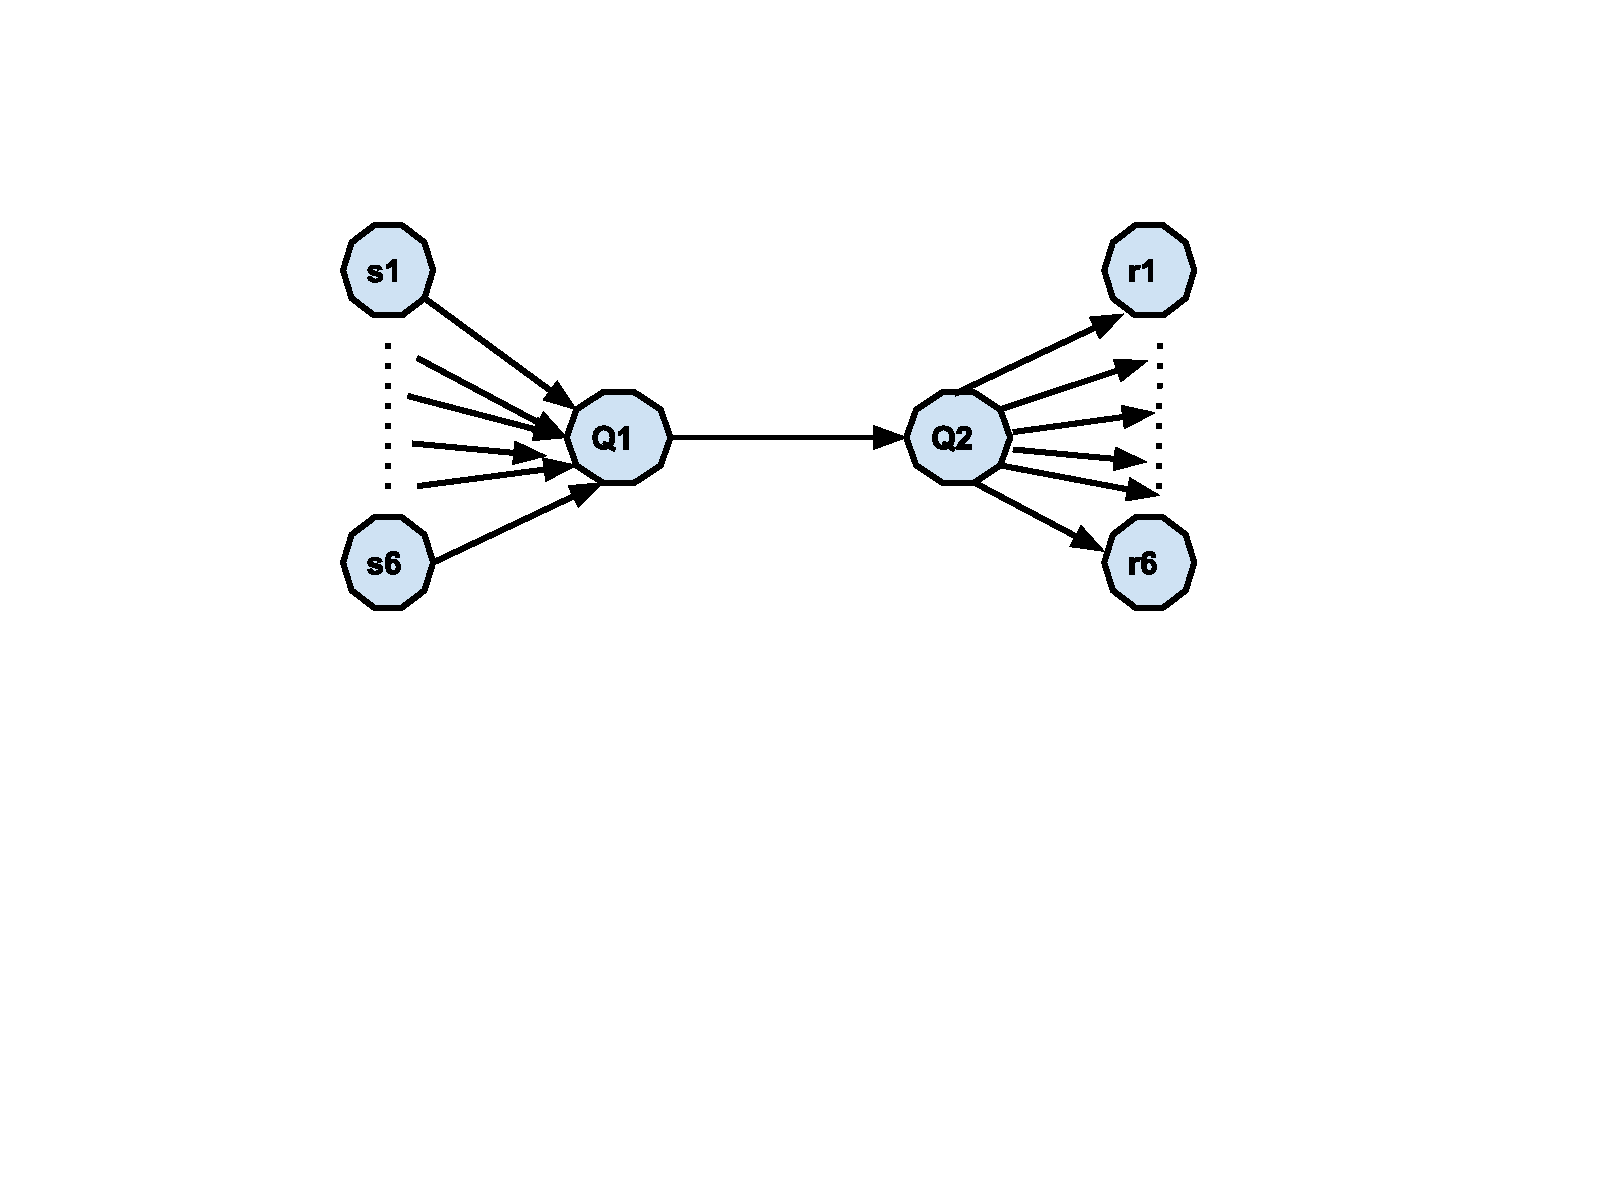
\includegraphics[width=6cm]{6layout.pdf}
\caption{Network topology}
\label{layout}
\end{figure}
\begin{itemize}
\item $6$ traffic senders and $6$ receivers.
\item The sender $s_{i}$ sends data to receiver $r_{i}$ through the bottleneck link $Q1\to Q2$. 
\item Both $Q1$ and $Q2$ maintain DropTail Queues. 
\item The queue limit is set to be the bandwidth-delay product to ensure the full utilization of the link capacity.
\end{itemize}
\end{frame}
\begin{frame}
\frametitle{End-user Data Collection Cont'd}
Without losing of generality, we simulated several different traffic scenarios to collect end-user data. We analyze the following scenarios: 
\begin{itemize}
    \item Scenario 1: All traffic sources are running TCP NewReno with stationary bottleneck link capacity.
    \item Scenario 2: All traffic sources are running TCP Cubic with stationary bottleneck link capacity.
    % \item Scenario 3: One half traffic sources are running TCP NewReno while the other half running TCP Cubic with stationary bottle link capacity.
    \item Scenario 3: One-half of the traffic sources is running TCP NewReno while the other half is running UDP with stationary bottleneck link capacity.
    \item Scenario 4: One-half of the traffic sources is running TCP Cubic while the other half is running UDP with stationary bottleneck link capacity.
    \item Scenario 5: Repeat scenario 1 and 2 for a periodically On-Off bottleneck link.
\end{itemize}
\end{frame}

\begin{frame}
\frametitle{Feature Set}
\begin{table}
\begin{center}
\caption {Simulation Parameters} \label{tab:simuPara}
\begin{tabular}{ |c|c| }
 \hline
 Access Link Capacity & 1Gbps  \\
 \hline
 BottleNeck Link Capacity & 1Gbps  \\
 \hline
 Access Link Delay & 5ms  \\
 \hline
 BottleNeck Link Delay & 10ms\\
 \hline
 Queue Capacity & Bandwidth-Delay Product\\
 \hline
\end{tabular}
\end{center}
\end{table}
\begin{itemize}
\item The sending time interval between two consecutive packets $T_{s_{i}}$.
\item The receiving time interval between two consecutive ACKs $T_{r_{i}}$.
\item An EWMA of $T_{s_{i}}$ (send\_ewma).
\item An EWMA of $T_{r_{i}}$ (ack\_ewma).
\item The ratio between the most recent RTT and the minimum RTT during the entire connection period (rtt\_ratio).
\end{itemize}

\end{frame}

\begin{frame}
\frametitle{Receiver Operating Characteristic (ROC) Curves}
 \begin{columns}[c]
 \column{.5\textwidth}
\begin{figure}
\centering
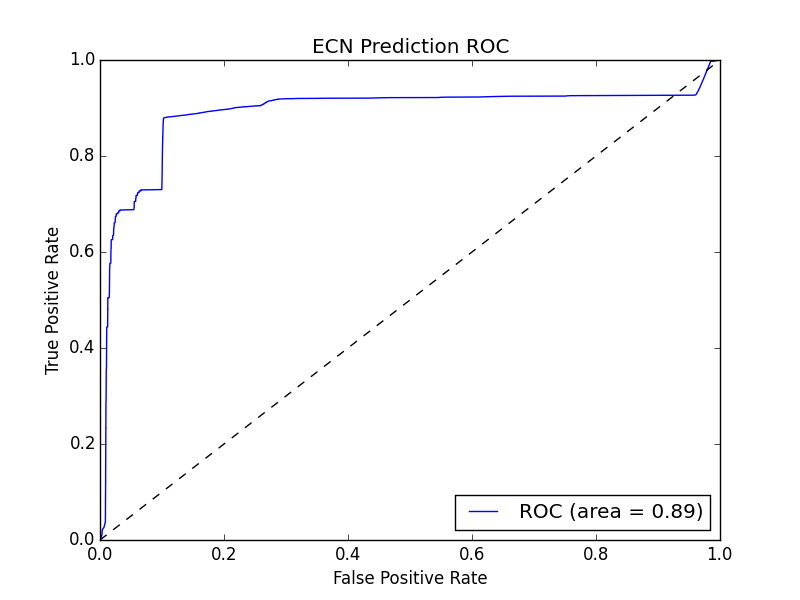
\includegraphics[width=5cm]{LRRoc.png}
\caption{ROC curve of the Logistic Regression classifier}
\label{LRRoc}
\end{figure}
 \column{.5\textwidth}
 \begin{figure}
     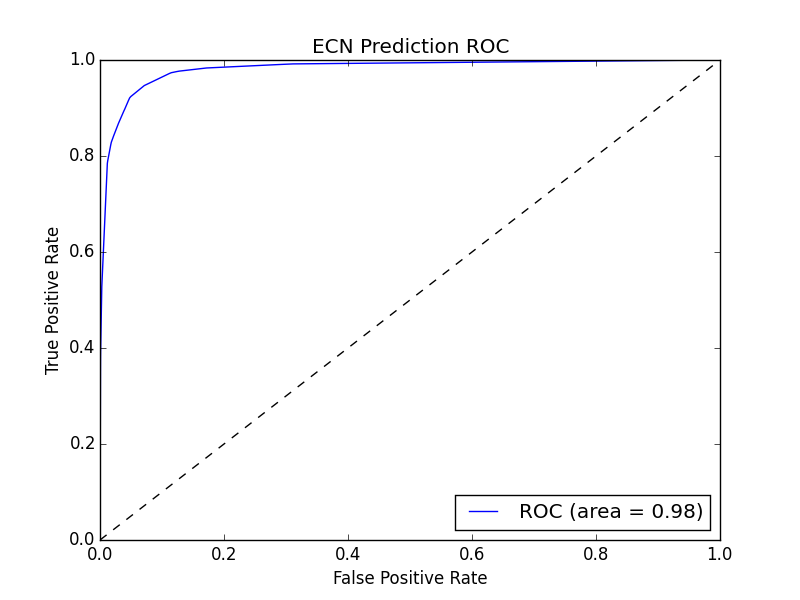
\includegraphics[width=5cm]{DecisionTreeRoc.png}
\caption{ROC curve of the Decision Tree classifier (max\_depth = 5, min\_samples\_leaf = 10000)}
\label{DecisionTreeRoc}

   \end{figure}
\end{columns}
\begin{itemize}
\item Logistic Regression: the decision boundary is $ -2.32*f_{1} - 33.36*f_{2} - 12.65*f_{3} - 15.30*f_{4} + 2.03*f_{5} - 2.69 = 0$.
\item Decision Tree: the feature importance is given as [$0.011703$, $0.00085$, $0.000000$, $0.03985$, $0.94760$].
\end{itemize}
\end{frame}
\begin{frame}
\frametitle{Receiver Operating Characteristic (ROC) Curves}
\begin{table}
\begin{center}
\caption {Simulation Parameters} \label{tab:varyRTT}
\begin{tabular}{ |c|c| }
 \hline
 Access Link Delay & 5ms, 10ms, 20ms  \\
 \hline
 BottleNeck Link Delay & 10ms, 20ms, 40ms\\
 \hline
 Queue Capacity & Bandwidth-Delay Product\\
 \hline
\end{tabular}
\end{center}
\end{table}
 \begin{columns}[c]
 \column{.5\textwidth}
\begin{figure}
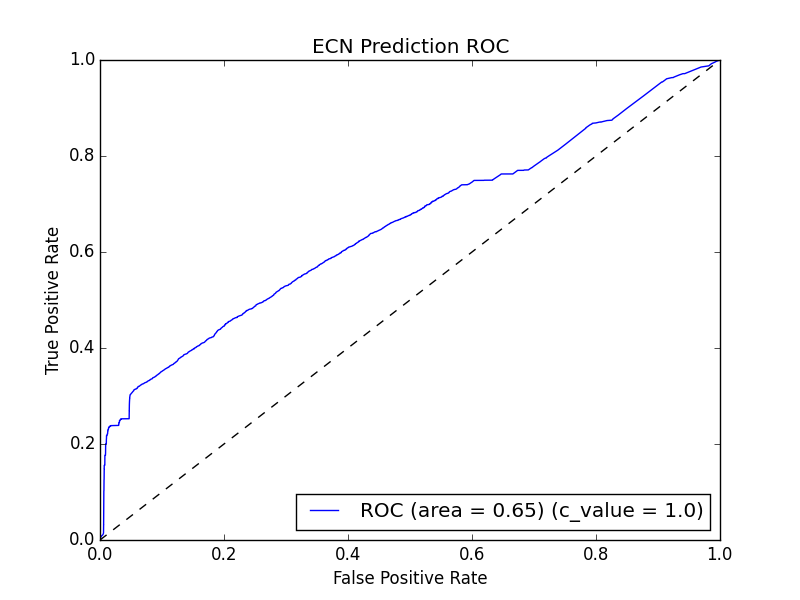
\includegraphics[width=4cm]{LRRocDiffProp.png}
\caption{ROC curve of Logistic Regression classifier with different propagation delays}
\label{LRROCDiff}
\end{figure}
 \column{.5\textwidth}
\begin{figure}
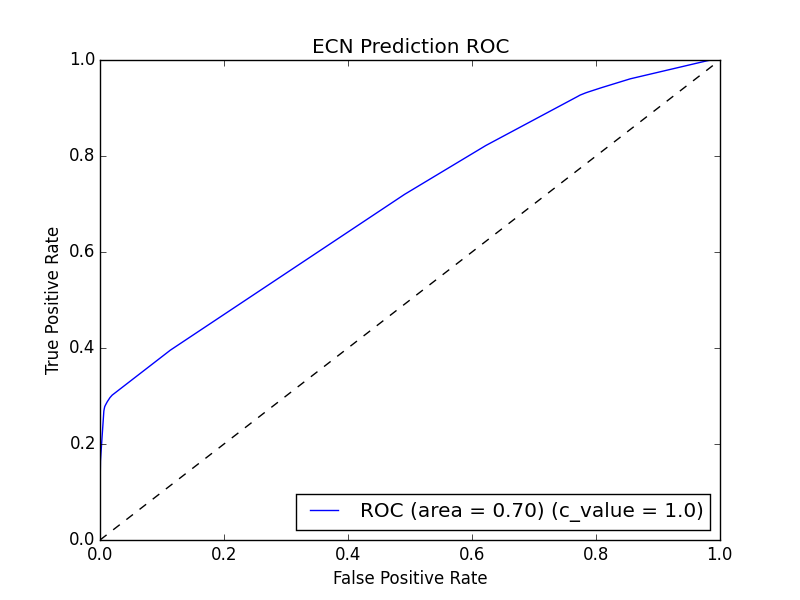
\includegraphics[width=4cm]{DTRocDiffProp.png}
\caption{ROC curve of Decision Tree classifier with different propagation delays}
\label{DTROCDiff}
\end{figure}
\end{columns}


\end{frame}
\section{Conclusions and Future Work}
\begin{frame}
\frametitle{Conclusions}
Conclusions:
\begin{itemize}

\item Cooperative communication can be used to mitigate correlated shadow fading, reduce outage frequency and probability of long-lasting outage durations. 
\item A first-order Markov Chain Model can be constructed to analyze the system performance under exponential correlated shadow fading.
\item The performance of a multi-cell system is investigated from the outage probability and outage durations. Connecting to the BS providing highest SINR or increasing the BS density can improve the system performance.
\item A data-driven end-user congestion detection algorithm is developed for stable networks.
\end{itemize}
\end{frame}
\begin{frame}
\frametitle{Future Work}
Future Work:
\begin{itemize}
\item Apply our algorithms to mitigate correlated shadow fading to the standard mmWave channel.
\item Use the proposed fast end-user congestion prediction algorithm to design fast reacting TCP congestion control algorithms for stable networks.
\item Extract new features and apply powerful machine learning algorithms to design fast reacting TCP congestion control algorithms for unstable networks.
\end{itemize}
\end{frame}
\begin{frame}
\frametitle{Publications}
Publications:
\begin{itemize}
\item "Shining a Light into the Darkness: How Cooperative Relay Communication Mitigates Correlated Shadow Fading", Accepted by VTC 2015 Spring.
\item "How Long Before I Regain My Signal?", Accepted by CISS 2015.
\end{itemize}
Technical Report:
\begin{itemize}
\item "Virtual ECN: A Data-Driven End-User Congestion Prediction Algorithm".
\end{itemize}
\end{frame}
%\section{High Throughput End-to-End TCP Congestion Control Protocol Design for 5G}
%\begin{frame}
%\frametitle{Motivations and Goals}
%Motivations
%\begin{itemize}
%\item 5G mmWave cellular networks are different from conventional cellular networks.
%\item Traditional TCP congestion control protocol does not give high end-to-end throughput given this new kind of communication network.
%\end{itemize}
%Goals
%\begin{itemize}
%\item Design a transport layer protocol optimized for the mmWave access network and for the new class of applications that it will enable.
%\item This protocol will have to work seamlessly across a connection consisting of both wireline and wireless segments.
%\end{itemize}
%\end{frame}
%
%\begin{frame}
%\frametitle{TCP}
%\begin{figure}
%\includegraphics[width=8cm]{tcp.png}
%\end{figure}
%\end{frame}
%\subsection{Channel Modeling of 5G mmWave Channel}
%\begin{frame}
%\frametitle{Markov Chain Model}
%\begin{figure}
%\includegraphics[width=8cm]{markov.png}
%\end{figure}
%\begin{itemize}
%\item To approximate the mmWave channel, a dummy Markov Chain Model will be constructed.
%\item Three states: Outage (state 0), Low Data Rate (state 1) and High Data Rate (state 2).
%\item State Transition Matrix:\[\left(\begin{array}{ccc}
%P_{00} & P_{01} & P_{02}\\
%P_{10} & P_{11} & P_{12}\\
%P_{20} & P_{21} & P_{22}\end{array}\right)\]
%\end{itemize}
%\end{frame}
%\subsection{Data Center TCP and Virtual ECN}
%\begin{frame}
%\frametitle{Vritual ECN}
%Instead of get the router involved to send the ECN, an end-to-end virtual ECN is generated.
%\begin{figure}
%\includegraphics[width=8cm]{procedure.png}
%\end{figure}
%\end{frame}
%\section{Future Work}
%\begin{frame}
%\frametitle{Future Work}
%\begin{itemize}
%\item Construct a Markov Chain Model to approximate the angular and distance model.
%\item Use this model to study the system performance.
%\item Construct a Markov Chain Model to mimic the 5G mmWave channel.
%\item Test the designed TCP congestion control protocol and improve it.
%\end{itemize}
%\end{frame}
\begin{frame}
\frametitle{The End}
\begin{centering}
THANKS!\\
QUESTIONS?\\
\end{centering}
\end{frame}
%\begin{frame}
%\begin{centering}
%HAPPY CHINESE LUNAR NEW YEAR!\\
%YEAR of the SHEEP or the GOAT!\\
%\end{centering}
%\begin{figure}
%\includegraphics[width=6cm]{year-of-the-sheep.jpg}
%\end{figure}
%\end{frame}
\end{document} 